% LaTeX Template for short student reports.
% Citations should be in bibtex format and go in references.bib
\documentclass[a4paper, 11pt]{article}
\usepackage[top=3cm, bottom=3cm, left = 2.5cm, right = 3cm]{geometry}
\usepackage[english]{babel} 
\geometry{a4paper} 
\usepackage[utf8]{inputenc}
\usepackage{textcomp}
\usepackage{graphicx} 
\usepackage{amsmath,amssymb} 
\usepackage{mathtools} 
\usepackage{bm}  
\usepackage[hidelinks]{hyperref} 
\usepackage{float}
\usepackage{algpseudocode}
\usepackage{algorithm}
\usepackage{parskip}
\usepackage{float}
\usepackage{subfig}
\usepackage{setspace}

\usepackage{caption}
\usepackage{lipsum}

\DeclareCaptionFormat{algor}{%
  \hrulefill\par\offinterlineskip\vskip1pt%
    \textbf{#1#2}#3\offinterlineskip\hrulefill}
\DeclareCaptionStyle{algori}{singlelinecheck=off,format=algor,labelsep=space}
\captionsetup[algorithm]{style=algori}




\usepackage{setspace}
\onehalfspacing

\usepackage{pgfplots}
\pgfplotsset{width=10cm,compat=1.9}

% \setlength{\parindent}{0cm}
%\hypersetup{linkcolor=black,citecolor=black,filecolor=black,urlcolor=black} % black links, for printed output
\usepackage{memhfixc} 
\usepackage{pdfsync}  
\usepackage{fancyhdr}
\pagestyle{fancy}

\usepackage[compact]{titlesec}  
\titlespacing*{\section}{0pt}{10ex plus 1ex minus .2ex}{4.3ex plus .2ex}

\usepackage[backend=biber, maxbibnames=99]{biblatex}


\usepackage{amsthm}


\newtheorem*{example*}{Example}
\newtheorem*{definition*}{Definition}

\clubpenalty = 10000
\widowpenalty = 10000
\displaywidowpenalty = 10000




\addbibresource{references.bib}

\title{Runtime analysis of the Java implementation of the CYK-algorithm}
\author{Pina Kolling \\ piko0011@student.umu.se}
%\date{}


\newcommand{\dq}{"}






%---------------------------------------------------------------------%

%---------------------------------------------------------------------%






\begin{document}


\begin{titlepage}
	\centering
	{\scshape\LARGE Ume\r{a} University \par}
	Efficient Algorithms \par
	\vspace{1cm}
	{\scshape\Large Report\par }
	\vspace{1.5cm}
	{\huge\bfseries  Runtime analysis of the Java implementation of the CYK-algorithm \par}
	\vspace{2cm}
	{\Large\itshape Pina Kolling\par}
	\vfill

% Bottom of the page
	{\large \today\par}
\end{titlepage}



%---------------------------------------------------------------------%








\section*{Abstract}

Formal languages and grammars can be used in different fields, for example for AI learning methods. The CYK-algorithm is a method to examine if an input word is part of a formal language. 
In this report, the implementation of different parsing methods for the CYK-algorithm is described. The runtimes of those methods are analysed and compared. For each method experiments with different inputs are documented and evaluated. The results of the experiments and the theoretical runtime analysis in $O$-notation are compared to show the differences and similarities. The results are also shown in graphs.
In addition to this, one method is modified to work with linear grammars and concepts of error correction are described and presented. 









%---------------------------------------------------------------------%




% \singlespacing


\setcounter{page}{1}

%\renewcommand{\baselinestretch}{0.9}\normalsize
%\tableofcontents

\begin{spacing}{1}


\newpage
\fancyhead[LO]{\empty}
{
  \hypersetup{linkcolor=black}
  \tableofcontents
}

\end{spacing}
% \doublespacing

\newpage

%\renewcommand{\baselinestretch}{1.3}\normalsize






%---------------------------------------------------------------------%








\section{Introduction}

Parsing in Computer Science is the process  of reading, analysing and processing an input string. In this context it is used for analysing a string of characters to examine if the string is built according to the rules of a formal grammar. 

A formal grammar describes how to form strings with correct syntax out of characters from a formal language's alphabet (explained in Section \ref{formalgrammar} and \ref{formallanguage}).
To examine if such a string follows the rules of a grammar, the \textit{Cocke-Younger-Kasami}-algorithm (short: \textit{CYK}) can be used. This algorithm is described in Section \ref{cyk}. To use the \textit{CYK}-algorithm, the grammar needs to be in a specific format, that is called \textit{Chomsky-Normal-Form} (short: \textit{CNF}), which is explained in Section \ref{cnf}. \cite{CYK_name, CYK1}


Three different parsing methods are implemented and described of which one executes the \textit{CYK}-algorithm with dynamic programming in \textit{Java}. The different parsing methods are described and presented as pseudo code in Section \ref{systemdesign}.
For the implementation three different classes are implemented: \texttt{main.java, grammar.java} and \texttt{parser.java}. The \texttt{main}-class calls the methods and the \texttt{grammar}-class parses the input grammar as string into a format that then can be processed in the \texttt{parser}-class. This \texttt{parser}-class has three different parsing methods, which are tested and compared against each other.
The function and implementation is former described in Section \ref{systemdesign}. Also in Section \ref{systemdesign} the runtimes in $O$-notation are calculated for each approach and modifications for the parsing of linear grammars are described.

In Section \ref{evaluation} the runtimes and experiments of the different algorithms are compared and differences in efficiency are shown. The results from the experiments are compared to the calculated runtimes in $O$-notation from Section \ref{systemdesign} and those differences are explained.

Concepts, ideas and first steps for the error correction of input words with deletion and exchange are presented in Section \ref{errorcorrection}.


In the final part (Section \ref{conclusion}) the results and future possibilities are discussed.




\pagebreak






%---------------------------------------------------------------------%








\section{Background}

In this section background information, definitions and examples on formal languages, alphabets and Kleene star (Section \ref{formallanguage}), formal grammars (Section \ref{formalgrammar}), Chomsky-Normal-Form (Section \ref{cnf}), CYK-algorithm (Section \ref{cyk}), dynmaic programming (Section \ref{dp}), recursion (Section \ref{recursion}) and divide and conquer (Section \ref{divide_and_conquer}) are presented. 

%---------------------------------------------------------------------%

\subsection{Formal language}
\label{formallanguage}


Formal languages are abstract languages, which define the syntax of the words that get accepted by that language. It is a set of words that get accepted by the language and has a set of symbols that is called alphabet, which contains all the possible characters of the words. Those characters are called nonterminal symbols. \cite{CNF, language}

\begin{definition*}[Kleene star]
The Kleene star $\Sigma^*$ of an alphabet $\Sigma$ is the set of all words that can be created through concatenation of the symbols of the alphabet $\Sigma$. The empty word $\epsilon$ is included. 
\end{definition*}

\begin{definition*}[Formal language]
A formal language $L$ over an alphabet $\Sigma$ is a subset of the Kleene star of the alphabet: $L \subseteq \Sigma^*$
\end{definition*}


\begin{example*}[Formal language]\footnote{The following examples show the \textit{Well-Balanced Parantheses} example from the assignment task sheet with the alphabet $\{a, b\}$ instead of $\{(, )\}$. } The language accepts words that contain the same amount of $a$s and $b$s, while the a has to be left of the b. 
The alphabet $\Sigma$ of this language looks like this:
\begin{align*}
\Sigma & = \{ a, b\}
\end{align*}
The Kleene star $\Sigma^*$ of the alphabet $\Sigma$ looks like this:
\begin{align*}
\Sigma^* & = \{ \epsilon, a, b, aa, ab, ba, bb, aaa, aab, abb, bbb, bba, baa, aba, bab, ...   \}
\end{align*}
The language definition $L$ is the following one:
\begin{align*}
L = \{ (a^{n}b^{n})^m \} \text{ with } n, m \in \mathbb{N}
\end{align*}

\end{example*}



%---------------------------------------------------------------------%

\subsection{Formal grammar}
\label{formalgrammar}


A formal grammar describes how to form strings with correct syntax from a language's alphabet. A grammar does not describe the meaning of the strings or any semantics — only their syntax is defined. The grammar is a set of rules, which define which words are accepted by a formal language. Those rules consist of terminal and nonterminal symbols. The terminal symbols are the characters of the alphabet of the language and the nonterminal symbols are used to build the rules of the language -- they get replaced by terminal symbols. \cite{CNF, language} 

\begin{definition*}[Formal grammar]
A formal grammar $G$ is defined as a 4-tuple:
\begin{align*}
G = (V, T, P, S)
\end{align*}
The set $V$ contains the nonterminal symbols of the grammar and the set $T$ the terminal symbols, which is the alphabet of a language. This assumes that $V \cap T = \emptyset$. The set $P$ is the set of production rules, where an element of $V$ points to an element of $V^* \times T^*$. The symbol $S \in V$ represents the start symbol. 

The production rules in the set $P$ have the format \texttt{head $\rightarrow$ body}. The head is always a nonterminal symbol and the body can be a combination of terminal and nonterminal symbols. A nonterminal symbol \texttt{A} in the body of a rule can be replaced by the body of a rule with the form \texttt{A $\rightarrow$ body}.
\cite{LS_Ulm}

A formal grammar defines which words over the alphabet $T$/$Sigma$ are contained in the associated laguage.
\end{definition*}

\begin{example*}[Formal grammar]
The example grammar $G$ for the previous example language $L$ over the alphabet $\Sigma$ is the following:
\begin{align*}
G = (\{S\}, \{ a, b \}, \{ S \rightarrow SS, S \rightarrow  aSb, S \rightarrow ab \},  \{ S \})
\end{align*}
The rules of the grammar $G$ over the alphabet $\{a, b\}$ with the start symbol $S$ and the nonterminal symbols $\{ S \}$ can also be written in the following form:
\begin{center}
\texttt{S $\rightarrow$ SS $\mid$  aSb $\mid$ ab}
\end{center}
The start symbol \texttt{S} can for example be replaced with its body \texttt{SS}. If then both symbols \texttt{S} are replaced with the body \texttt{ab} the resulting word is \texttt{abab}. It is part of the language, because it was build with the grammar $G$.
\end{example*}

%---------------------------------------------------------------------%

\subsection{Chomsky-Normal-Form}
\label{cnf}

The \textit{Chomsky-Normal-Form} (short: \textit{CNF}) is a grammar which is formatted in a specific way. If the head of a rule (nonterminal symbol) is not generating the empty word (\textit{\texttt{S $\rightarrow \epsilon$}}) it either generates two nonterminal symbols or one terminal symbol for the grammar to be in \textit{CNF}.
\cite{CNF}

\begin{example*}[Chomsky-Normal-Form]
This is the previous example in CNF. How it was built can be seen in Appendix \ref{createcnf}.
\begin{align*}
\texttt{S} & \rightarrow \texttt{SS} \mid  \texttt{LA} \mid \texttt{LR} \\
\texttt{A} & \rightarrow \texttt{SR} \\
\texttt{L} & \rightarrow a \\
\texttt{R} & \rightarrow b
\end{align*}
\end{example*}


%---------------------------------------------------------------------%

\subsection{Dynamic programming}
\label{dp}

The technique of dynamic programming can be used to solve problems, which can be divided into smaller subproblems. The solutions of the subproblems are saved (for example in a multi-dimensional array) and referenced later. \cite{DP}
\\
\begin{example*}[Knapsack problem]

As an example the table for the knapsack problem is filled out, because it is a really common example for the concept of dynamic programming.
\\ \\
Given is a set of items with a weight and a value. The task is to choose which items to include so that the total weight is less than the given limit of the knapsack and the total value is as large as possible.
\\ \\
The formula with which the dynamic programming works is the following:


  $$
Opt(i,j)=
\begin{cases}
0, & \text{for } 0\leq j \leq size\\
        Opt(i-1, j), & \text{for } j < w[i]\\
        max\{ Opt(i-1, j), v[i]+Opt(i-1, j-w[i]) \}, & \text{else } 
\end{cases}
$$

If $0 \leq j \leq w$ then there are no objects which could be put into the bag. The second case acts when object $i$ does not fit into the bag and the optimal solution is found with the objects from index $1$ to $i-1$. Else the object $i$ is either part of the optimal solution or it consists out of the objects $1$ to $i-1$.


The table of the values and weight of each item with index $i$ is shown on the left and on the right is the table that gets filled in with a dynamic programming approach of the formula above. The maximum bag size is 7.
\\ \\
\begin{minipage}{0.3\textwidth}

\begin{tabular}{|c|c|c|}
\hline
$i$ & $w[i]$ & $v[i]$ \\
\hline
1 & 1 & 1 \\
2 & 3 & 4 \\
3 & 2 & 3 \\
4 & 4 & 6 \\
5 & 6 & 8 \\
\hline
\end{tabular}


\end{minipage}\begin{minipage}{0.1\textwidth}
\ 
\end{minipage}\begin{minipage}{0.6\textwidth}

\begin{tabular}{|c||c|c|c|c|c|c|c|c|}
\hline
5 & 0 & 1 & 3 & 4 & 6 & 7 & 9 & 10 \\
\hline
4 & 0 & 1 & 3 & 4 & 6 & 7 & 9 & 10 \\
\hline
3 & 0 & 1 & 3 & 4 & 5 & 7 & 8 & 8 \\
\hline
2 & 0 & 1 & 1 & 4 & 5 & 5 & 5 & 5 \\
\hline
1 & 0 & 1 & 1 & 1 & 1 & 1 & 1 & 1 \\
\hline
0 & 0 & 0 & 0 & 0 & 0 & 0 & 0 & 0 \\
\hline
\hline
  & 0 & 1 & 2 & 3 & 4 & 5 & 6 & 7 \\
\hline

\end{tabular}

\end{minipage}
\ \\

The first column in the table represent the objects and the last row the weight. The entries in the table show the maximum value. In this example the maximum value for the size 7 is 10.


\end{example*}


%---------------------------------------------------------------------%

\subsection{CYK-algorithm}
\label{cyk}


\textit{Cocke-Younger-Kasami}-algorithm (short: \textit{CYK}-algorithm) takes a grammar $G = (V, T, P, S)$ in \textit{CNF} and a word $w= w_1, w_2, ..., w_n \in T^*$ as an input. It then examines if the word follows the rules of the grammar. Then for every substring $w_{i, j} = w_i, ..., w_{i+j-1}$ (begins at index $i$ and has the length $j$) of the word $w$  the set of nonterminal symbols that lead to $w_{i, j}$ gets calculated and saved as $V_{i, j}$ to access it in later steps. \cite{CYK1}


\begin{example*}[Chomsky-Normal-Form]
The following table shows the CYK-algorithm with the previous grammar example and the input word $aaabbb$. 
The word is accepted by the grammar rules, because the initiating nonterminal symbol \textit{\texttt{S}} can be filled into the lowest field. The table is filled in step by step and the rules that are used in each step are marked, for a better understanding on how the algorithm works. \cite{cyk_online_alg}
\ \\

\begin{center}
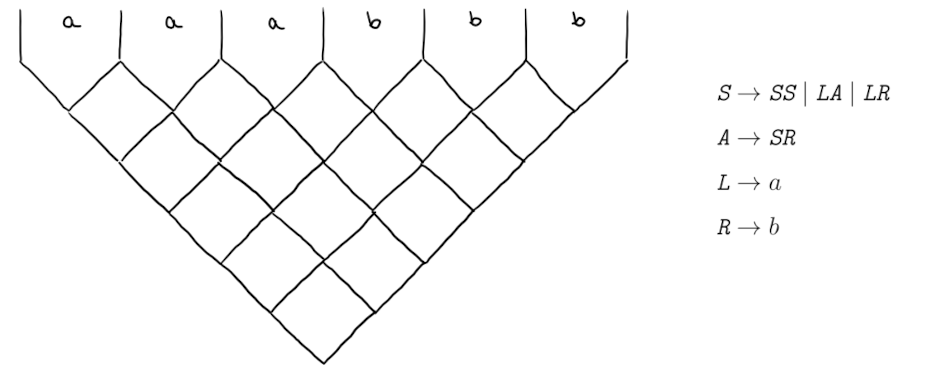
\includegraphics[scale=0.9]{images/7.png} \\
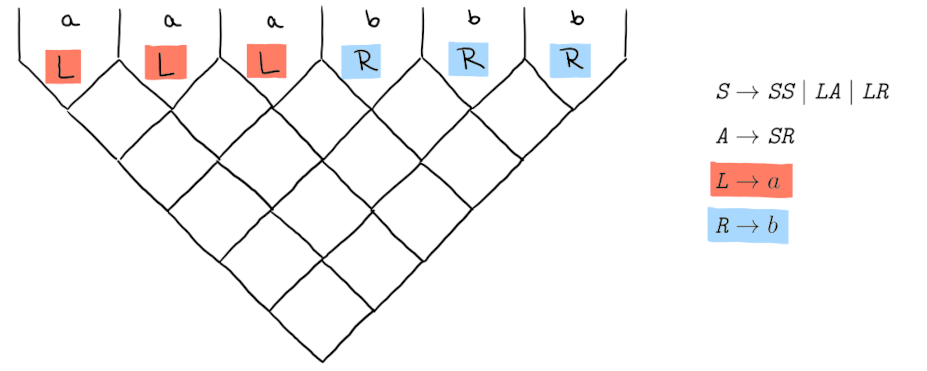
\includegraphics[scale=0.9]{images/6.png} \\
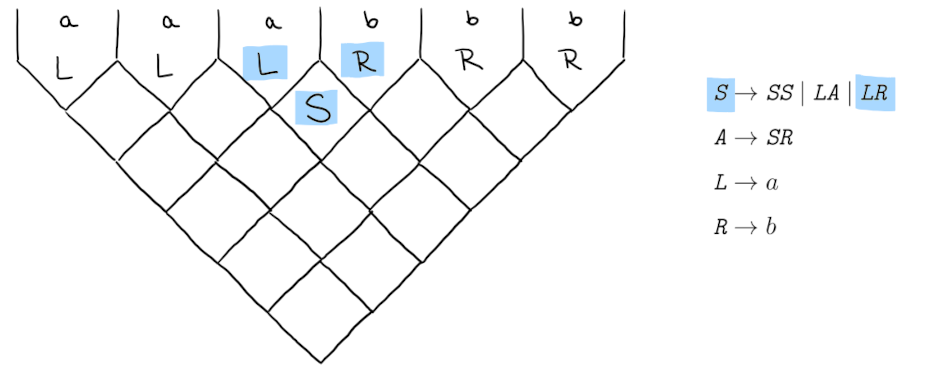
\includegraphics[scale=0.9]{images/5.png} \\
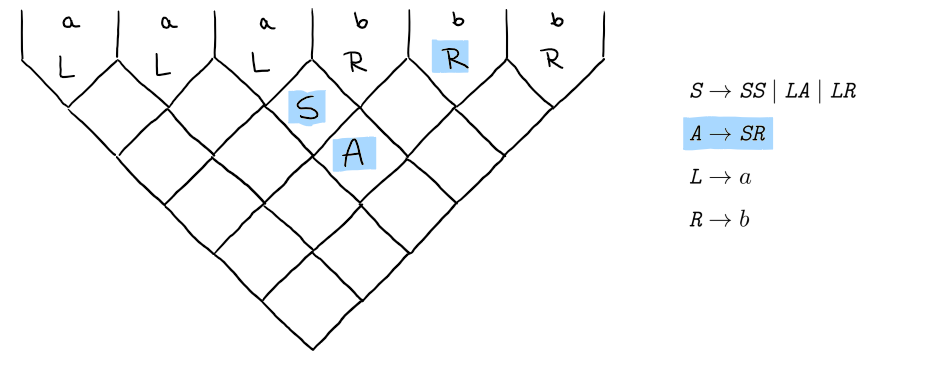
\includegraphics[scale=0.9]{images/4.png} \\
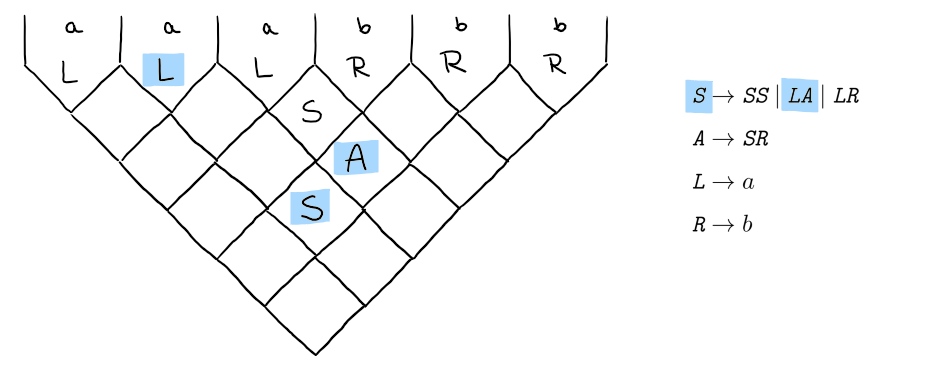
\includegraphics[scale=0.9]{images/3.png} \\
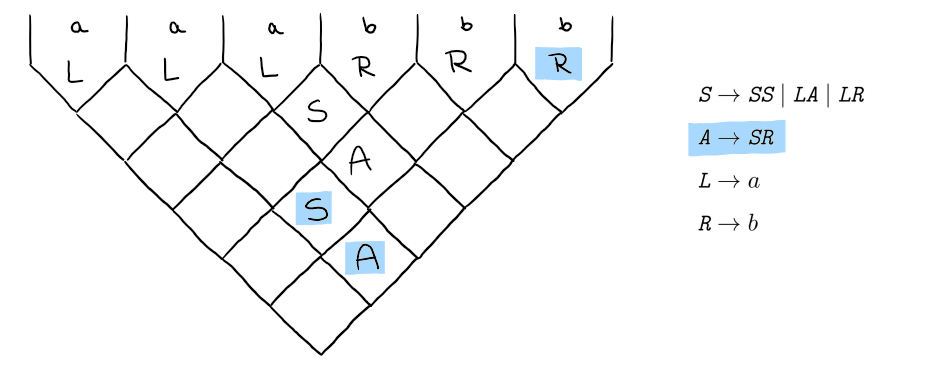
\includegraphics[scale=0.9]{images/2.png} \\
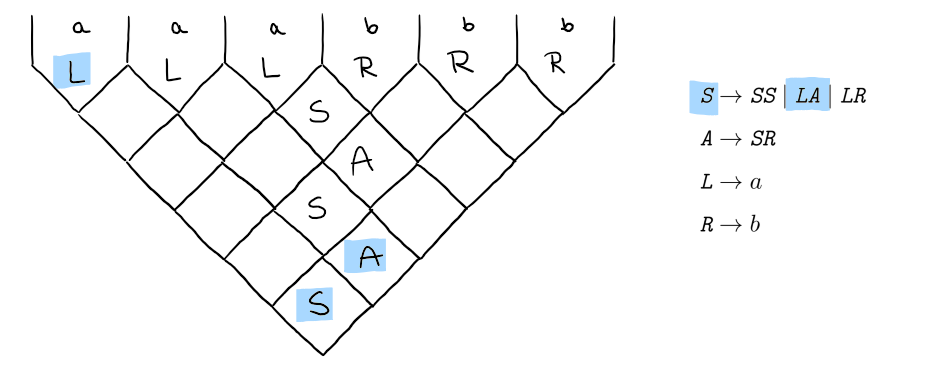
\includegraphics[scale=0.9]{images/1.png} \\
\end{center}
% \caption{CYK-algorithm step by step table for the word $aaabbb$}

\end{example*}



%---------------------------------------------------------------------%

\subsection{Recursion}
\label{recursion}

A function that calls itself is called recursive function. In computer science recursive functions use base cases to terminate the program and stopping it from going on forever. Base cases are problems that can be solved without any more recursive calls.
\cite{recursion}

\begin{example*}[Recursion]

For definition and examples for recursion read Section \ref{recursion}.

\end{example*}


\begin{example*}[Recursion]
Building a sum for the numbers $1+2+...+n$.

Nonrecursive approach:
\begin{align*}
f(n) = 1+2+...+n
\end{align*}

Recursive approach:
\begin{align*}
f(n) = 1 \ \ \ \ \ \ \ \ \ \ \ \ \ \ \  & \ \ \ \text{if } n=1 \\
f(n) = n + f(n-1) & \ \ \ \text{if } n > 1
\end{align*}

\end{example*}


\subsection{Divide and conquer}
\label{divide_and_conquer}

The divide and conquer method is used to design efficient algorithms. In this method, the problem is divided recursively into smaller and simpler subproblems, until those subproblems can be solved. Then those subproblems are combined again to give the solution of the original problem.

\begin{example*}[Divide and conquer]

A problem that can be solved with divide and conquer is the sorting of an array. The array is then divided in smaller arrays, until the array size is one. Then the subarrays are merged together in the correct order.

The unsorted array for the example is the following:
\begin{center}
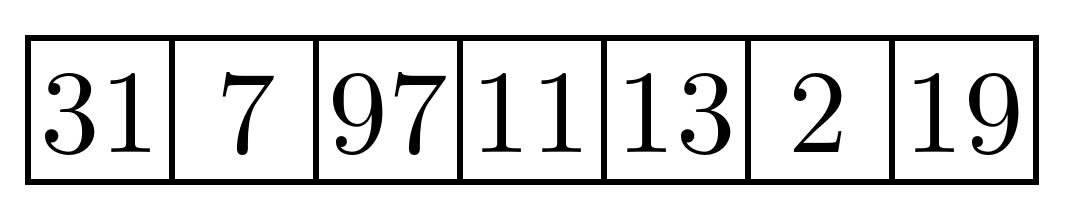
\includegraphics[scale=0.125]{images/merge1.png}
\end{center}

The array gets divided into two smaller subarray, which are sorted with the same technique individually and later merged together again:
\begin{center}
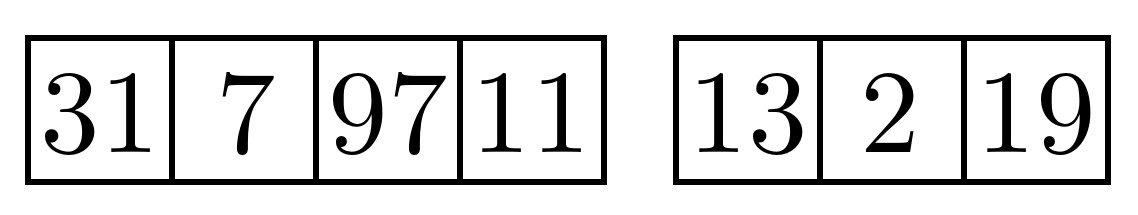
\includegraphics[scale=0.125]{images/merge2.png}
\end{center}

Those subarrays get divided into even smaller arrays again:
\begin{center}
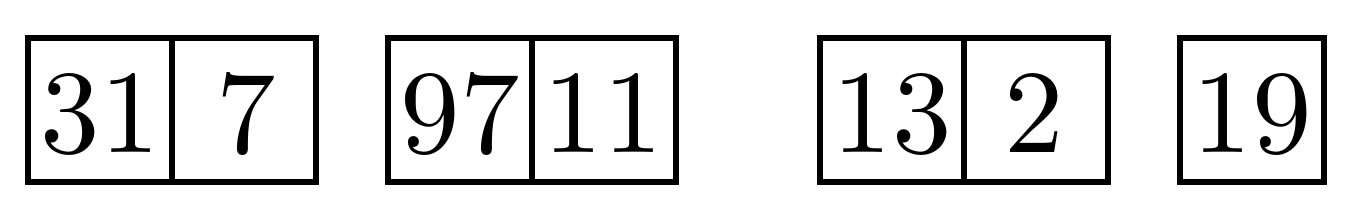
\includegraphics[scale=0.125]{images/merge3.png}
\end{center}

The array size of the subproblems is now 1:
\begin{center}
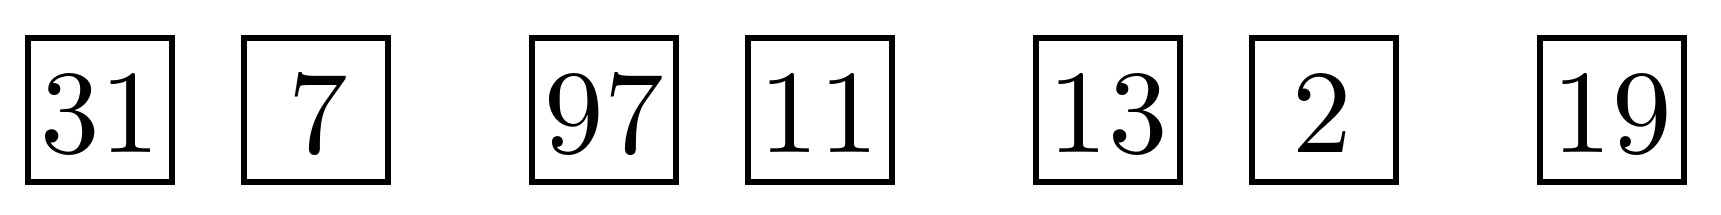
\includegraphics[scale=0.125]{images/merge4.png}
\end{center}

The subarrays get merged together in the right order:
\begin{center}
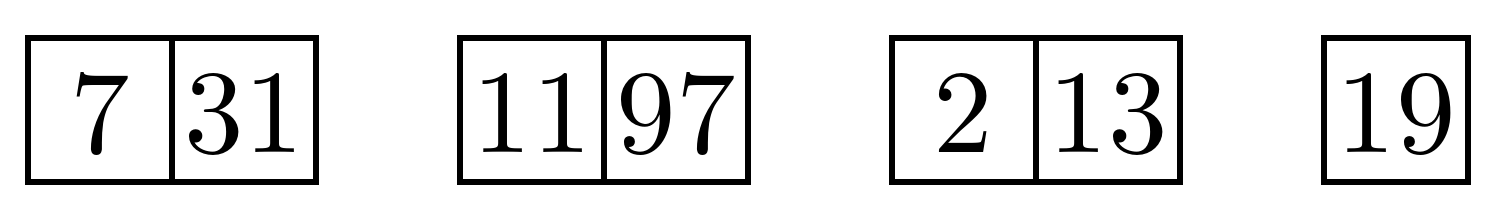
\includegraphics[scale=0.125]{images/merge5.png}
\end{center}

\newpage
For each merge of the subarrays only the smallest symbols of each array need to be compared. The smaller one is then sorted into the merged array and again the smallest symbols are compared:
\begin{center}
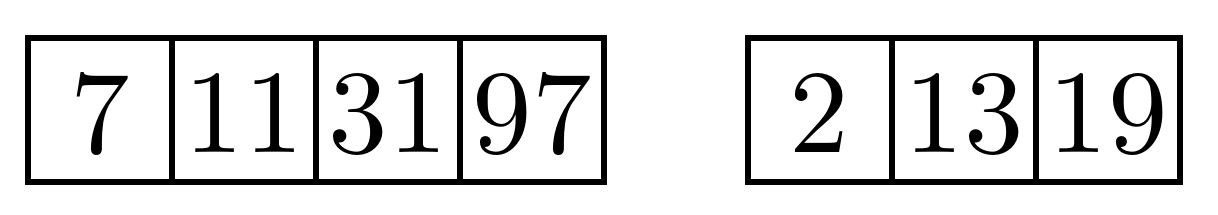
\includegraphics[scale=0.125]{images/merge6.png}
\end{center}

The array is complete and sorted:
\begin{center}
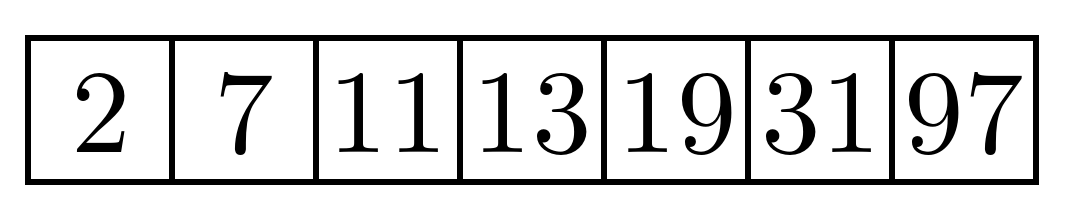
\includegraphics[scale=0.125]{images/merge7.png}
\end{center}


\end{example*}



%---------------------------------------------------------------------%



\pagebreak





%---------------------------------------------------------------------%








\section{Three variants of CYK algorithm}
\label{systemdesign}

The implementation was done in Java and three different classes were implemented: \texttt{main.java} (described in Section \ref{main}), \texttt{grammar.java} (described in Section \ref{grammar}) and \texttt{parser.java} (described in Section \ref{parser}). The \texttt{main}-class calls the methods and the \texttt{grammar}-class parses the input grammar and string into a format that then can be processed in the \texttt{parser}-class.


%---------------------------------------------------------------------%



\subsection{Main}
\label{main}

The \texttt{main}-class takes the input grammar and word and parses them into \texttt{String[]} and \texttt{String}. 
A detailed description on how to run the code can be found in Appendix \ref{howtousethecode}.


%---------------------------------------------------------------------%
%---------------------------------------------------------------------%

\subsection{Grammar}
\label{grammar}


The \texttt{grammar}-class assigns the nonterminal symbols to integers and builds arrays with them. The arrays have the type \texttt{Integer[][][]}. The start symbol for example is then assigned with the integer zero and the bodies of that rule are at the index zero of the three-dimensional array. The first dimension represents the head of a rule, the second dimension represents the body which is divided into two arrays -- for each symbol of the body one array.


For faster and easier access, three arrays are built: One array that only contains nonterminal symbols and rules, one array that contains only terminal rules and one array that contains both.








%---------------------------------------------------------------------%
%---------------------------------------------------------------------%

\subsection{Parser}
\label{parser}

The \texttt{parser}-class contains three different parsing methods: \texttt{parseNaive} (described in Section \ref{naivedescription}), \texttt{parseTopDown} (described in Section \ref{topdowndescription}) and \texttt{parseBottomUp} (described in Section \ref{bottomupdescription}). Also there exists a modified method of the \texttt{parseTopDown}, which takes linear grammars (which are translated into \textit{CNF}) and parses them faster (described in Section \ref{lineartopdown}).

Each method has a counter as \texttt{long} which counts the number of iterations and a timer as \texttt{long} in $ms$ which measures the runtime of the method. In the following sections the algorithms are described, presented as pseudo code and the runtime is analysed.

%---------------------------------------------------------------------%

\subsubsection{Naive description}
\label{naivedescription}

% TODO: describe idea of algorithm more detailed in text form!

The naive algorithm is a recursive divide-and-conquer algorithm. The problem gets divided into smaller subproblems and then the method is called again for each subproblem. It returns a boolean and has an initial method to start the recursion with the start values:
\begin{itemize}
\item The start symbol of the grammar is first parameter. It is an integer called \texttt{indexNT} and initialized with 0, because the start symbol is assigned to the index 0.
\item The second parameter is the integer 0 as a start index of the input word.
\item The third parameter is the integer $n$, which is the length of the input word.
\end{itemize} 


The start values get assigned in the recursion call which can be seen in the following pseudo code:
 
\begin{center}
\captionof{algorithm}{Recursion call: Boolean parseNaive()}\label{alg:cap}
\label{alg_naive_rec_call}
\begin{algorithmic}[1]
\State $counter \gets 0$
\State \Return parseNaive(0, 0, inputWord.length)
\end{algorithmic}
\hrulefill
\end{center}

The naive approach does not use dynamic programming. Instead it checks for each call \texttt{parseNaive(indexNT, i, j)} first if $i = j-1$ and checks if the nonterminal symbol head of \texttt{indexNT} leads to a body of a rule with \texttt{s[i]}. This is the base case of the recursion which then returns true or false depending if the rule \texttt{indexNT $\rightarrow$  s[i]} exists. This base case can be seen in line 2-7 in the pseudo code below.
\\ 
\\
If $i$ is not equal to $j-1$ it loops for the integer $k$ from $i+1$ to $j-1$ and checks for all rules \texttt{A $\rightarrow$ BC} if both calls \texttt{parseNaive(B, i, k)} and \texttt{parseNaive(C, k, j)} return true. This recursive call applies the function on the substrings of the input word. If such a pair of substrings is found, the function returns true, because the recursive call in combination with the \grqq \texttt{and}\grqq \ leads to the result of the complete word. If such a pair cannot be found the function returns false after looping through all rule bodies and values for $k$. This part of the recursion can be seen in the pseudo code below in line 9-21.





\begin{center}
\captionof{algorithm}{Boolean parseNaive(int indexNT, int i, int j)}\label{alg:cap}
\begin{algorithmic}[1]
\State $counter \gets counter+1$
\If{$i == (j-1)$}
\For{$l \gets 0$ \textbf{to} $ruleset[0].length$}
\If{$ruleset[indexNT][l][0] == inputWord[i]$ \newline \hspace*{5em} \textbf{or}  $ruleset[indexNT][l][1] == inputWord[i]$}
\State \Return true
\EndIf
\EndFor

\Else
\For{$bodyIndex \gets 0$ \textbf{to} $ruleset[indexNT].length$}
\If{$ruleset[indexNT][bodyIndex][0] \  != null$ \newline \hspace*{5em} \textbf{and} $ruleset[indexNT][bodyIndex][1] \  != null$}
\State $first \gets ruleset[indexNT][bodyIndex][0]$
\State $second \gets ruleset[indexNT][bodyIndex][1]$
\For{$k \gets i+1$ \textbf{to} $j$}
\If{$parseNaive(first, i, k)$ \textbf{and} $parseNaive(second, k, j)$}
\State \Return true
\EndIf
\EndFor
\EndIf
\EndFor
\EndIf
\State \Return false
\end{algorithmic}
\hrulefill
\end{center}

\subsubsection{Naive runtime}
\label{naiveruntime}

In the following table the upper bound runtime of the second method (algorithm 2) is listed for each line. The variable $n$ represents the length of the input word and $k$ the dimension of the rule array.
\ \\ \ \\
\begin{minipage}{0.5\textwidth}

\begin{tabular}{|c|c|l|}
\hline
Line & Runtime & Type \\
\hline
1 &  $1$ & Assignment \\
2 &  $1$ & Comparison \\
3 & $k$  & Loop \\
4 & $1$ $\cdot$ $k$ & Comparison \\
5 & $1$ $\cdot$ $k$ & Return statement\\
9 & $k$ & Loop \\
10 & $1$ $\cdot$ $k$ & comparison \\
11 & 1 $\cdot$ $k$ & Assignment \\
12 & 1 $\cdot$ $k$ & Assignment\\
13 & n $\cdot$ $k$ & Loop \\
14 & $n!$ & Recusrsive call \\
15 & $1$ $\cdot$ $n$ $\cdot$ $k$ & Return statement\\
21 & $1$ & Return statement \\
\hline
\end{tabular}

\end{minipage}\begin{minipage}{0.5\textwidth}
Calculating the runtime:
\vspace*{-1em}
\begin{align*}
& 1 + 1+ k + k +k + k + k + k + k \\
& + n \cdot k + n^n + n \cdot k \\
& =  2 + 7k + 2(n \cdot k) + n! \\
& = 2 + 7k + 2n \cdot 2k + n! \\
& \in O(n!)
\end{align*}
The runtime of the naive method is in $O(n!)$.
\end{minipage}

%---------------------------------------------------------------------%


\subsubsection{Top-Down description}
\label{topdowndescription}

% TODO: describe idea of algorithm more detailed in text form!

The top-down method is an improved version of the naive method (Section \ref{naivedescription}). This algorithm works recursive and with the concept of divide and conquer, too. In this algorithm another global array is used, which contains the values \texttt{true}, \texttt{false} and \texttt{null}. The array gets initialized with \texttt{null} in each field. That happens in the recursion call method below.

\begin{center}
\captionof{algorithm}{Recursion call: Boolean parseTD()}\label{alg:cap}
\begin{algorithmic}[1]
\State $counter \gets 0$
\For{$i \gets 0$ \textbf{to} $table.length$ }
\For{$j \gets 0$ \textbf{to} $table[i].length$}
\For{$k \gets 0$ \textbf{to} $table[i][j].length$}
\State $table[i][j][k] \gets null$
\EndFor
\EndFor
\EndFor
\State \Return parseTD(0, 0, inputWord.length)
\end{algorithmic}
\hrulefill
\end{center}

Additional to the naive algorithm, the recursion in the topdown approach starts with another condition: If one of the values in the global table is not \texttt{null}, the next recursive call is not executed and this value gets returned. This if-condition can be seen in the following part of the pseudo code. The rest of the topdown approach is a similar approach to the naive method that was already described in Section \ref{naivedescription}.

\begin{center}
\captionof{algorithm}{Additional condition in Boolean parseTD(int indexNT, int i, int j)}\label{alg:cap}
\begin{algorithmic}[1]
\If{table[indexNT][i][j] \ != null}
\State \Return table[indexNT][i][j]
\EndIf
\end{algorithmic}
\hrulefill
\end{center}

The complete topdown algorithm is shown as pseudo code below. In the inner for-loop (line 18) the boolean value of the next method calls get assigned into the global table. If there is assigned a true (line 19) the value true gets returns (lime 20). The general topdown approach is the same approach as the naive method that is described in Section \ref{naivedescription}.

\begin{center}
\captionof{algorithm}{Boolean parseTD(int indexNT, int i, int j)}\label{alg:cap}
\begin{algorithmic}[1]
\State $counter \gets counter+1$
\State $rulesetLength \gets ruleset[0].length$
\If{$table[indexNT][i][j] \  != null$}
\State \Return $table[indexNT][i][j]$
\EndIf
\If{$i == (j-1)$}
\For{$l \gets 0$ \textbf{to} $ruleset[0].length$}
\If{$ruleset[indexNT][l][0] == inputWord[i]$ \newline \hspace*{5em} \textbf{or}  $ruleset[indexNT][l][1] == inputWord[i]$}
\State \Return true
\EndIf
\EndFor

\Else
\For{$bodyIndex \gets 0$ \textbf{to} $ruleset[indexNT].length$}
\If{$ruleset[indexNT][bodyIndex][0] \  != null$ \newline \hspace*{5em} \textbf{and} $ruleset[indexNT][bodyIndex][1] \  != null$}
\State $first \gets ruleset[indexNT][bodyIndex][0]$
\State $second \gets ruleset[indexNT][bodyIndex][1]$
\For{$k \gets i+1$ \textbf{to} $j$}
\State $table[indexNT][i][j] \gets (parseTD(first,i,k)$ \texttt{and} $parseTD(second,k,j))$
\If{$table[indexNT][i][j] == true$}
\State \Return true
\EndIf
\EndFor
\EndIf
\EndFor
\EndIf
\State \Return false
\end{algorithmic}
\hrulefill
\end{center}

\subsubsection{Top-Down runtime}
\label{topdownruntime}

In this part the runtime of the topdown method is calculated.
The variable $n$ represents the length of the input word and $k$ the dimension of the rule array. The first part of the calculation shows the recursion call method.

\ \\ \\
\begin{minipage}{0.5\textwidth}

\begin{tabular}{|c|c|l|}
\hline
Line & Runtime & Type \\
\hline
1 &  1 & Assignment \\
2 & k & Loop \\
3 & k $\cdot$ n & Loop \\
4 & k $\cdot$ n $\cdot$ n &  Loop\\
5 & k $\cdot$ n $\cdot$ n $\cdot$ 1 & Assignment\\
9 & ... & Function call\\
\hline
\end{tabular}


\end{minipage}\begin{minipage}{0.5\textwidth}
Calculating the runtime of the method call:
\begin{align*}
& 1 + k + k \cdot n + k \cdot n \cdot n + k \cdot n \cdot n \\
& = 1 + k + k \cdot n + 2(n^2 \cdot k) \\
& \in O(n^2)
\end{align*}
\end{minipage}
\ \\

The runtime analysis for the upper bound of the \texttt{parseTD} method is analogue to the \texttt{parseNaive} runtime analysis. According to this the topdown algorithm has an upper bound runtime in $O(n!)$, too.



\subsubsection{Top-Down modified for linear grammars}
\label{lineartopdown}

For the parsing of linear grammars, the topdown approach (Section \ref{topdowndescription}) was modified to reduce the amounts of recursive calls. The topdown approach was chosen, because it seems to have the best performance of the different parsing methods, considering the experiments.

In the modified version for linear grammars, the grammar gets changed into CNF first. The modified algorithm can now work more efficient, because for each rule is only one recursive call of the method instead of two necessary.

For each rule it is checked if the first or the second element of the body is the head of a terminal rule. Then it is checked if the head of the terminal rule is the head of the current position on the input word. For the other symbol the methos gets called recursively. This part is shown in the pseudo code below:


\begin{center}
\captionof{algorithm}{boolean parseLinearTD(int indexNT, int i, int j)}
\begin{algorithmic}[1]
\State $counter \gets counter+1$
\State $rulesetLength \gets ruleset[0].length$
\If{$table[indexNT][i][j] \  != null$}
	\State \Return $table[indexNT][i][j]$
\EndIf
\If{$i == (j-1)$}
	\For{$l \gets 0$ \textbf{to} $ruleset[0].length$}
	\If{$ruleset[indexNT][l][0] == inputWord[i]$ \newline \hspace*{5em} 		\textbf{and}  $rulesetLinear[indexNT][l][1] == null$}
		\State $tableLinear[indexNT][i][j] \gets true$
		\State \Return true
	\EndIf
	\EndFor
	\State \Return false
\EndIf 

\For{$bodyIndex \gets 0$ \textbf{to} $ruleset[indexNT].length$}
	\If{$ruleset[indexNT][bodyIndex][0] \  != null$ \newline 					\hspace*{5em} \textbf{and} $ruleset[indexNT][bodyIndex][1] \  !			= null$}
		\State $first \gets ruleset[indexNT][bodyIndex][0]$
		\State $second \gets ruleset[indexNT][bodyIndex][1]$
		\For{$k \gets i+1$ \textbf{to} $j$}
			\If{\textit{second} is head of a terminal rule}
				\State{$table[indexNT][i][j] = parseLinearTD(first, i, 					k)$ \textbf{and} \textit{second} is head of 							terminal rule with body $inputAsInt[k]$}
			\EndIf
			\If{\textit{first} is head of a terminal rule}
				\State{$table[indexNT][i][j] = parseLinearTD(second, k, 				j)$ \textbf{and} \textit{first} is head of terminal 					rule with body $inputAsInt[i]$}
			\EndIf
		\EndFor
	\EndIf
\EndFor

\If{$tableLinear[indexNT][i][j] != null \textbf{ and } 						tableLinear[indexNT][i][j] == true$}
	\State \Return true
\EndIf

\State $tableLinear[indexNT][i][j] \gets false$
\State \Return false
\end{algorithmic}
\hrulefill
\end{center}


\subsubsection{Top-Down modified for linear grammars runtime}
\label{lineartopdown_runtime}

The runtime of the modified version is $O(n^2)$, because the recursive call is not in $O(n!)$ anymore like in Section \ref{naiveruntime} but $O(n)$. Instead the method is in $O(n^2)$.


%---------------------------------------------------------------------%


\subsubsection{Bottom-Up description}
\label{bottomupdescription}

The \texttt{parseBU} method works with dynamic programming.
First a table $DP$ with the size $n \times n$ gets constructed (line 2) -- $n$ represents the input word length.
In the first step the integers that represent the nonterminal symbols that are head of a terminal rule get assigned (line 3 - 12). For the character at index i of the input word the value of $DP[i][i]$ gets the nonterminal symbol that leads to the character of the word.
The approach of dynamic programming calculates the smallest substrings first and saves them for the efficient processing of the next bigger substrings.  The smallest substrings are the single characters.


\begin{center}
\captionof{algorithm}{Boolean parseBU()}\label{alg:cap}
\begin{algorithmic}[1]
\State $wordlength \gets word.length$ 
\State $Integer[][][] DP \gets new Integer[wordLength][wordLength][wordlength]$
\For{$i \gets 0$ \textbf{to} $wordlength$}
\If{$ruleset \ contains \ word[i]$}
\State assign nonterminal symbols of $inputword[i]$ to $DP[i][i]$
\EndIf
\EndFor

\For{$l \gets 0$ \textbf{to} $wordlength$}
\For{$i \gets 0$ \textbf{to} $wordlength - l$}
\State $j \gets i + l$
\For{$k \gets 0$ \textbf{to} $j$}

\For{$head \gets 0$ \textbf{to} $ruleset.length$}
\For{$body \gets 0$ \textbf{to} $ruleset[head].length$}
\State $conter \gets counter + 1$
\If{$ruleset[indexNT][bodyIndex][0] \  != null$ \newline \hspace*{5em} \textbf{and} $ruleset[indexNT][bodyIndex][1] \  != null$}
\State $first \gets ruleset[head][body].charAt[0]$
\State $second \gets ruleset[head][body][1]$
\If{$DP[i][k] \ contains \ first$ \textbf{and} $DP[k+1][j] \ contains \ second$}
\State assign head to $DP[i][j][c]$\footnotemark
\EndIf
\EndIf
\EndFor
\EndFor
\EndFor
\EndFor
\EndFor
\If{$DP[0][wordlength-1] \  contains \ 0$}
\State \Return true
\EndIf
\State \Return false
\end{algorithmic}
\hrulefill
\end{center}
\footnotetext{$c$ is the first empty position in $DP[i][j]$}

In line 13 to 32 the \textit{CYK}-algorithm gets executed. It is described in section \ref{cyk}. For each field the two fields \textit{leading} to it get compared, to then fill in the head of a rule that concludes into the both compared nonterminal symbols.


In the last lines (line 33-35) the last field of the $DP$-array gets checked. If it containes the start symbol of the grammar, the word is contained in the language and the algorithm returns true. Else false is returned.




\subsubsection{Bottom-Up runtime}
\label{bottomupruntime}

In the following part the upper bound runtime of the bottom up algorithm gets analysed.
The variable $n$ represents the length of the input word and $k$ the dimension of the rule array. \\

\begin{minipage}{0.6\textwidth}

\begin{tabular}{|c|c|l|}
\hline
Line & Runtime & Type \\
\hline
1 &  1 & Assignment \\
2 & 1 & Assignment \\
3 & n & Loop \\
4 &  n &  Comparison\\
5 & n  & Assignment\\
6 & n &  Comparison\\
7 & n &  Assignment \\
9 & n & Assignment \\
13 & n & Loop \\
14 & n $\cdot$ n& Loop\\
15  & n $\cdot$ n  & Assignment \\
16 & n $\cdot$ n $\cdot$ n & Loop \\
17  & n $\cdot$ n $\cdot$ n $\cdot$ k & Loop \\
18  & n $\cdot$ n $\cdot$ n $\cdot$ k $\cdot$ k & Loop \\
19 & n $\cdot$ n $\cdot$ n $\cdot$ k $\cdot$ k & Assignment\\
20 & n $\cdot$ n $\cdot$ n $\cdot$ k $\cdot$ k & Comparison\\
21 & n $\cdot$ n $\cdot$ n $\cdot$ k $\cdot$ k & Assignment\\
22& n $\cdot$ n $\cdot$ n $\cdot$ k $\cdot$ k & Assignment\\
23 & n $\cdot$ n $\cdot$ n $\cdot$ k $\cdot$ k & Comparison\\
24  & n $\cdot$ n $\cdot$ n $\cdot$ k $\cdot$ k & Assignment \\
25   & n $\cdot$ n $\cdot$ n $\cdot$ k $\cdot$ k & Assignment\\
33 & 1 & Comparison\\
34 & 1 & Return statement\\
36  & 1 &  Return statement\\
\hline
\end{tabular}


\end{minipage}\begin{minipage}{0.4\textwidth}
Calculating the runtime:
\begin{align*}
& 5 + 7n + 2n^2 + n^3 +n^3 \cdot k + 8 \cdot n^3 \cdot k^2 \\
& 5 + 7n + 2n^2 + (k+1)n^3 + 8 \cdot n^3 \cdot k^2 \\
& \in O(n^3)
\end{align*}

\end{minipage}
\ \\
The runtime of the \texttt{parseBU} method is in $O(n^3)$.


%---------------------------------------------------------------------%

\pagebreak






%---------------------------------------------------------------------%







\section{Evaluation}
\label{evaluation}

In this section the calculated runtimes in $O$-notation from Section \ref{systemdesign} and experiments are compared. 
First, in section \ref{experiments}, the results of different grammars and input words are presented in tables and as graphs.
In section \ref{runtime} the results of section \ref{experiments} and the calculated runtimes in $O$-notation from Section \ref{systemdesign} are compared.

More information and definitions on the $O$-notation can be read in \textit{Big O Notation} from P. Danziger \cite{bigO}.


\subsection{Experiments}
\label{experiments}

The following tables show some tests that were run with the different parsing methods and grammars. The first of each column for the method shows the truth value that is returned (as T for true and F for false), C represents the counter and T the time in ms.
\\
\\
\textbf{Well-Balanced-Parantheses:} \\
\texttt{"SSS" "SLA" "SLR" "ASR" "L(" "R)" "($^*$)$^*$"}

The Well-Balanced-Parantheses grammar accepts words, that contain a closed bracket \texttt{)} for each opened bracket \texttt{(}. The closed bracket has to appear after the accorsing opened bracket.

Different length and combinations of accepted input words were evaluated by the different parsing methods and the tables and graphs are shown below.

In the following table and graphs, variations of the input word \texttt{($^*$)$^*$} were evaluated.




\begin{small}
\begin{tabular}{|c|c||c|c|c||c|c|c||c|c|c|}
\hline
Word & Length & N & NC & NT & B & BC & BT & T & TC & TT \\
\hline
\hline
() & 2 & T & 6 & 5ms & T & 0 & 2ms & T & 6 & 1ms \\
\hline
(()) & 4 & T & 33 & 4ms & T & 84 & 3ms & T & 28 & 1ms \\
\hline
((())) & 6 & T & 212 & 6ms & T & 360 & 6ms & T & 84 & 1ms \\
\hline
(((()))) & 8 & T & 1295 & 6ms & T & 924 & 9ms & T & 190 & 1ms \\
\hline
((((())))) & 10 & T & 7666 & 9ms & T & 1872 & 11ms & T & 362 & 1ms \\
\hline
((...)) & 20 & T & 51.863.993 & 1.049ms & T & 15.732 & 23ms & T & 2.772 & 3ms \\
\hline
((...)) & 30 & T & 348.838.486.712 & 3.699.571ms & T & 102.660 & 32ms & T & 9.232 & 5ms \\
\hline
((...)) & 40 & & & & T & 127.452 & 50ms & T & 21.743 & 4ms \\
\hline
\end{tabular}
\end{small}

The input word with a length of $40$ did not terminate over night for the naive approach. The corresponding graphs to the data in the table are shown below. In the experiments with input words of a length of $8$ or smaller, the graphs show that the naive parser seems to perform the best. Considering longer input words, it can be observed, that the naive parser clearly has the most growth. This observations of the performance with short input words can be disregarded, because the amounts of calls for input words with a length smaller than $8$ do not have a big difference to each other. For the longer words, the results are showing more clearly.
\\
\begin{figure}[H]
\begin{center}
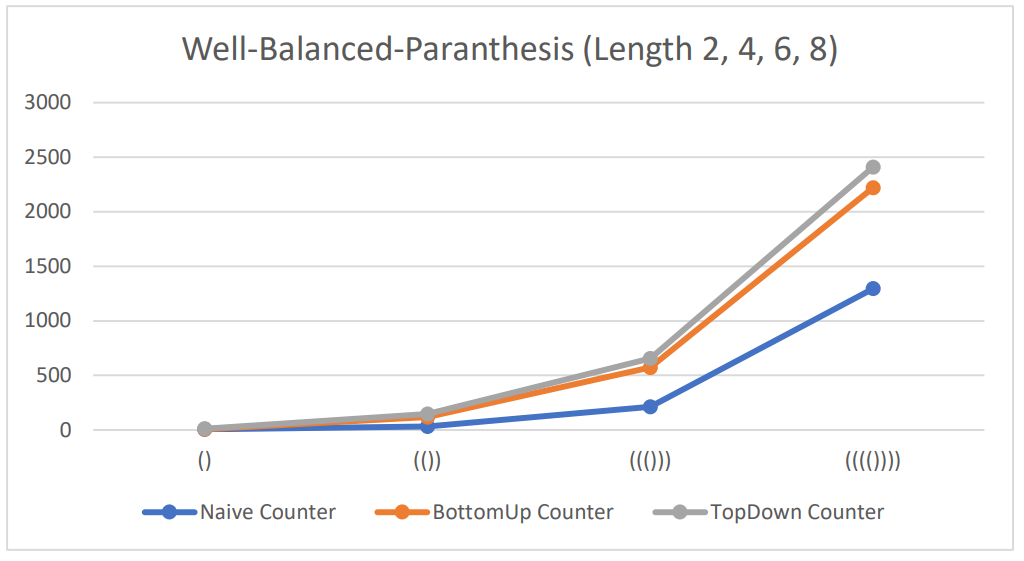
\includegraphics[scale=0.4]{diagrams/WBP_1.png}
\end{center}
\caption{Well-Balanced-Parantheses with input \texttt{()}, \texttt{(())}, \texttt{((()))} and \texttt{(((())))}}
\end{figure}

\begin{figure}[H]
\begin{center}
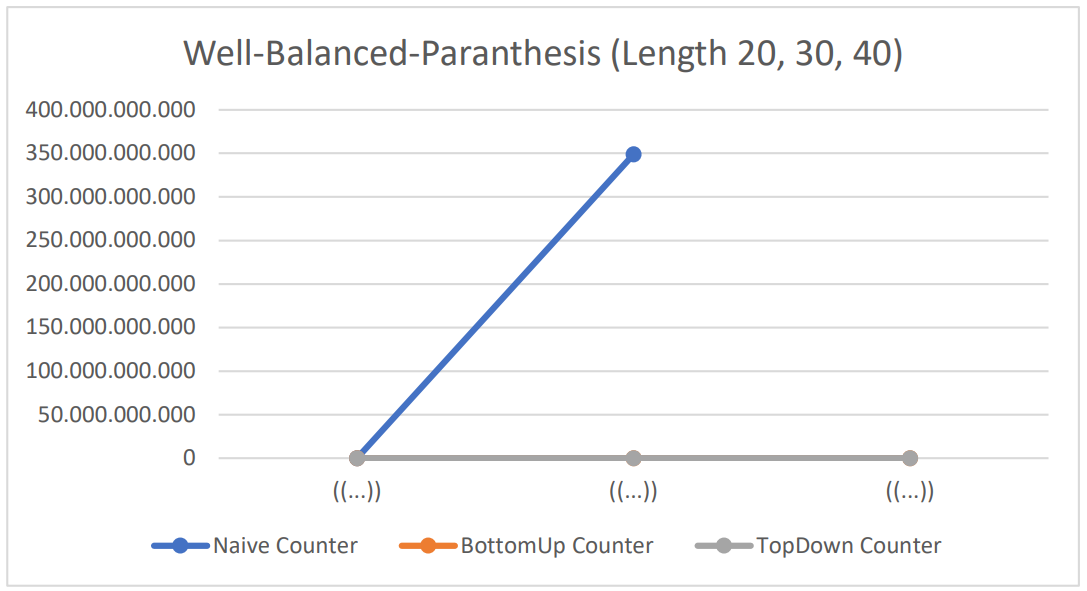
\includegraphics[scale=0.4]{diagrams/WBP_2.png}
\end{center}
\caption{Well-Balanced-Parantheses with input of length $20$, $30$ and $40$}
\end{figure}

In the following table and graphs, variations of the input word \texttt{(())$^*$} were evaluated.

\begin{small}
\begin{tabular}{|c|c||c|c|c||c|c|c||c|c|c|}
\hline
Word & Length & N & NC & NT & B & BC & BT & T & TC & TT \\
\hline
\hline
(()) & 4 & T & 33 & 0ms & T & 168 & 7ms & T & 28 & 5ms \\
\hline
(())(()) & 8 & T & 89 & 1ms & T & 1680 & 7ms & T & 60 & 2ms \\
\hline
(())(())(()) & 12 & T & 145 & 1ms & T & 6072 & 14ms & T & 92 & 3ms \\
\hline
(())(())(())(()) & 16 & T & 201 & 15ms & T & 14.880 & 13ms & T & 124 & 3ms \\
\hline
(())(())(())(())(()) & 20 & T & 257 & 15ms & T & 29.640 & 21ms & T & 156 & 4ms \\
\hline
(())(())(())(())(())(()) & 24 & T & 313 & 16ms & T & 51.888 & 22ms & T & 188 & 5ms \\
\hline

\end{tabular}
\end{small}

\begin{minipage}{0.45\textwidth}

\begin{figure}[H]
\begin{center}
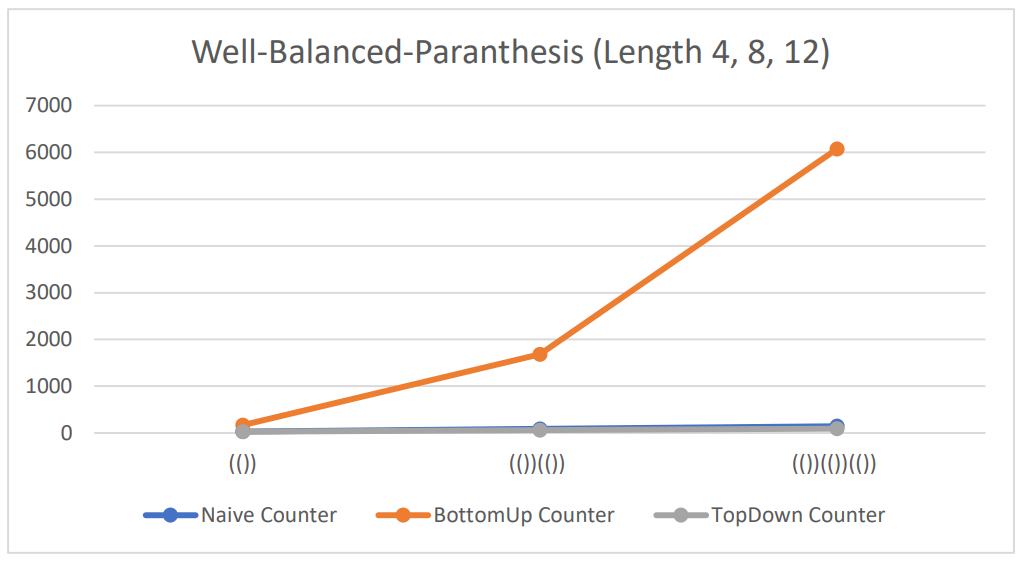
\includegraphics[scale=0.28]{diagrams/BP_1.png} 
\caption{Well-Balanced-Parantheses with input \texttt{(())}, \texttt{(())(())} and \texttt{(())(())(())}}
\end{center}

\end{figure}

\end{minipage}\begin{minipage}{0.1\textwidth}
\ 
\end{minipage}\begin{minipage}{0.45\textwidth}

\begin{figure}[H]
\begin{center}
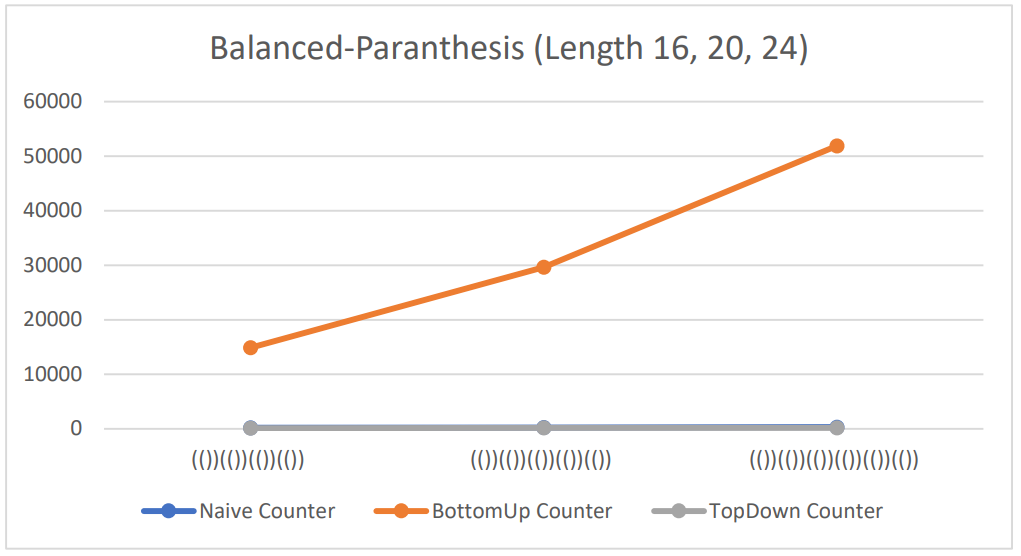
\includegraphics[scale=0.28]{diagrams/BP_2.png}
\caption{Well-Balanced-Parantheses with input words of length $16$, $20$ and $24$ \\ \ }
\end{center}

\end{figure}

\end{minipage}


\begin{figure}[H]
\begin{center}
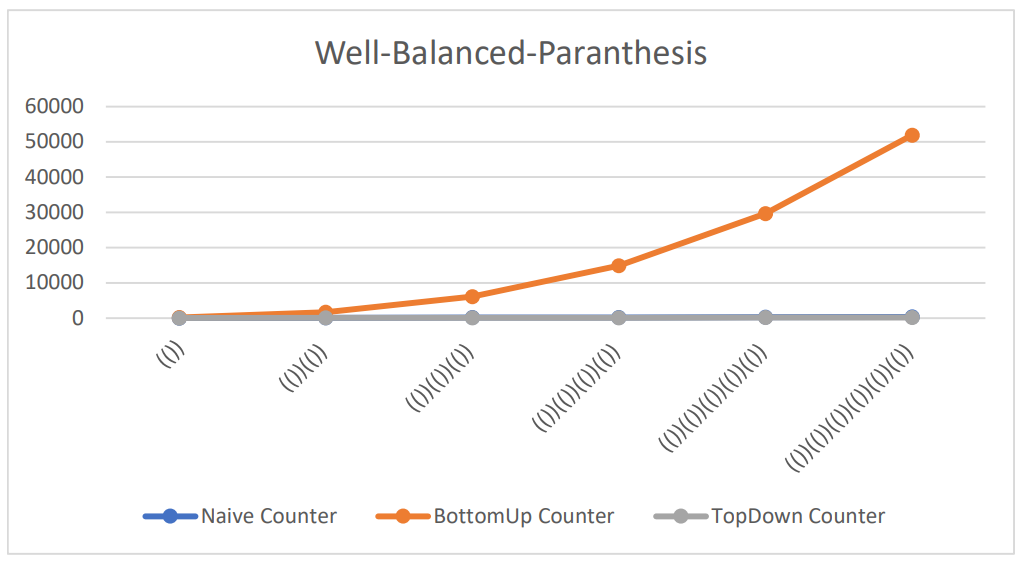
\includegraphics[scale=0.4]{diagrams/BP_C.png}
\end{center}
\caption{Well-Balanced-Parantheses with input of length $4$, $8$, $12$, $16$, $20$ and $24$ }
\end{figure}



\textbf{Stupid grammar:} \\
\texttt{"SST" "STS" "Ta"}

The stupid grammar accepts no input word, because the nonterminal symbol \texttt{S} cannot be resolved into a terminal symbol. The only terminal symbol of this grammar is the symbol \texttt{a}.

The input word with a length of $32$ did not terminate for the naive approach. The corresponding graphs to the data in the table are shown below.

\begin{tabular}{|c|c||c|c|c||c|c|c||c|c|c|}
\hline
Word & Length & N & NC & NT & B & BC & BT & T & TC & TT \\
\hline
\hline
a & 1 & F & 1 & 1ms & F & 0 & 6ms & F & 1 & 5ms \\
\hline
aa & 2 & F & 4 & 1ms & F & 4 & 8ms & F & 4 & 2ms \\
\hline
aaaa & 4 & F & 33 & 5ms & F & 28 & 6ms & F &27 & 1ms \\
\hline
aaaaaaaa & 8 & F & 1.596 & 8ms & F & 308 & 5ms & F & 197 & 1ms \\
\hline
aaaaaaaaaaaaaaaa & 16 & F & 3.524.577 & 89ms & F & 2.660 & 15ms & F & 1.481 & 1ms \\
\hline
aaaaaaa...aaaaaaaaa & 32 &  & & & F & 41.664 & 25ms & F & 11.409 & 4ms \\
\hline
\end{tabular}

The corresponding graphs to the data in the table are shown below. In the experiments with input words of a length of $4$ or smaller, the graphs show that the naive parser seems to perform the best. Considering longer input words, it can be observed, that the naive parser clearly has the most growth. This first observation of the naive parser performing the best can be disregarded, because the amounts of calls for input words with a length smaller than $4$ do not have a big difference to each other. For the longer words, the results are showing more clearly.


\begin{minipage}{0.45\textwidth}

\begin{figure}[H]
\begin{center}
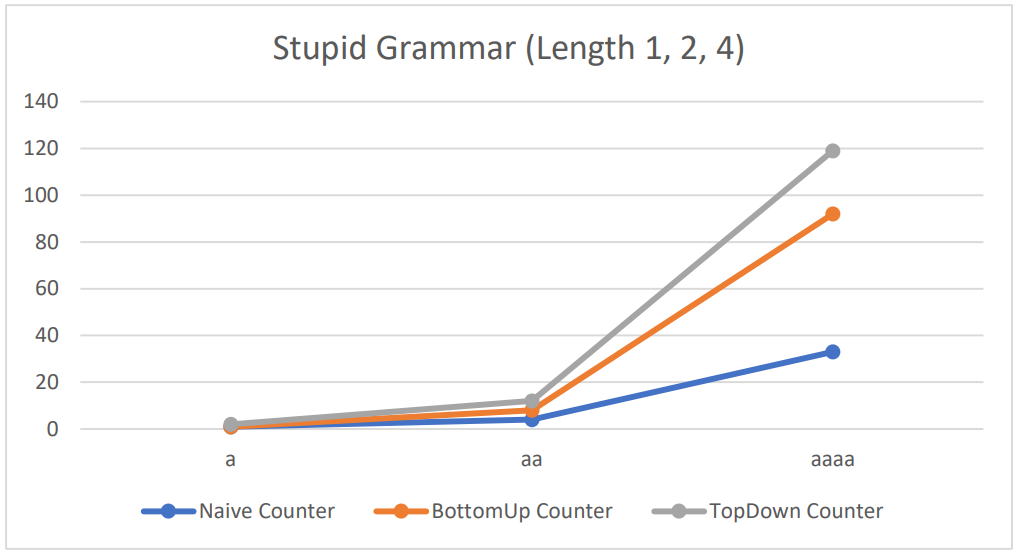
\includegraphics[scale=0.28]{diagrams/SG_1.png}
\end{center}
\caption{Stupid grammar with input \texttt{a}, \texttt{aa} and \texttt{aaaa}}
\end{figure}

\end{minipage}\begin{minipage}{0.1\textwidth}
\ 
\end{minipage}\begin{minipage}{0.45\textwidth}

\begin{figure}[H]
\begin{center}
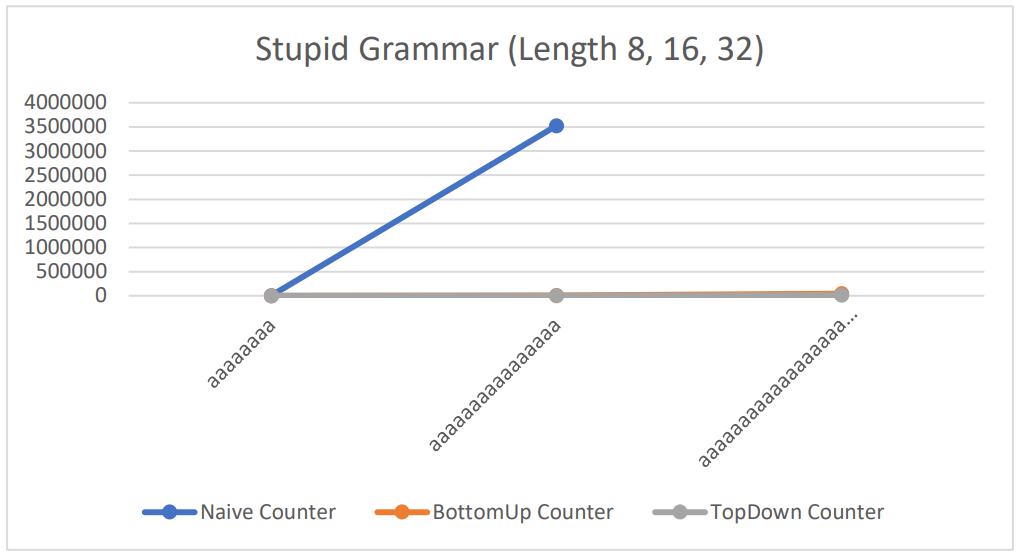
\includegraphics[scale=0.28]{diagrams/SG_2.png}
\end{center}
\caption{Stupid grammar with input of length $8$, $16$ and $32$}
\end{figure}

\end{minipage}


\begin{figure}[H]
\begin{center}
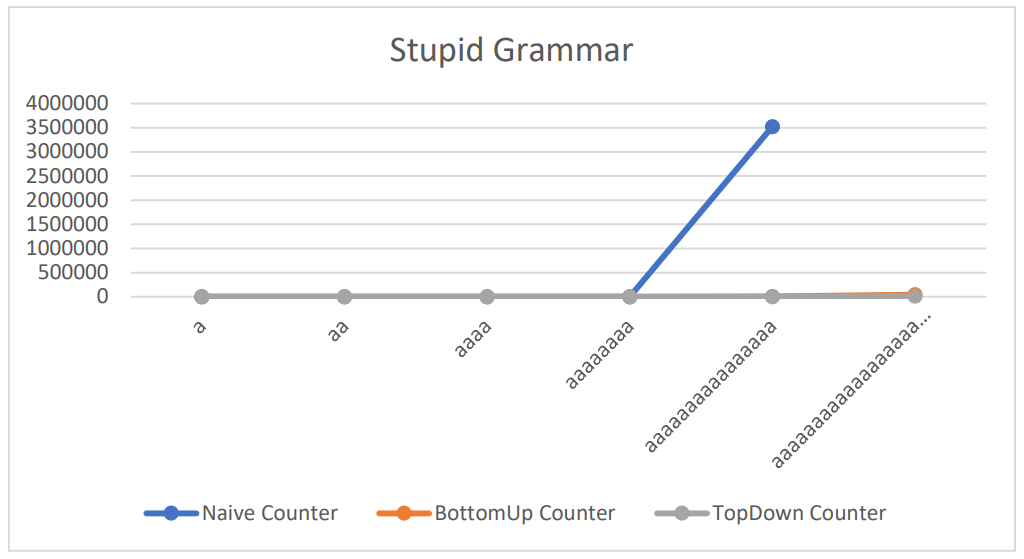
\includegraphics[scale=0.4]{diagrams/SG_C.png}
\end{center}
\caption{Stupid grammar with input of length $1$, $2$, $4$, $8$, $16$,  and $32$}
\end{figure}



%\textbf{Linear grammar example (abc-grammar):} \\
%\texttt{"SAc" "Sb" "AaS" "AaB" "BbS" "a$^*$b$^*$c$^*$"}
%\ \\ \\
%\begin{small}
%\begin{tabular}{|c|c||c|c||c|c||c|c||c|c|c|}
%\hline
%Word & Length & NC & NT & BC & BT & TC & TT & LC & LT \\
%\hline
%\hline
%abc & 3 & 6 & 1ms & 60 & 5ms & 6 & 3ms & 5 & 0ms \\
%\hline
%aabbcc & 6 & 51 & 1ms & 660 & 5ms & 49 & 3ms & 51 & 1ms \\
%\hline
%aaaabbbbcccc & 12 & 1.457 & 1ms & 6.072 & 9ms & 518 & 3ms & 650 & 1ms \\
%\hline
%a...b...c... & 24 & 481.557 & 9ms & 51.888 & 20ms & 4.312 & 4ms & 6.732 & 3ms \\
%\hline
%\end{tabular}
%\end{small}

%The incrementations of the input word length was chosen, to show the difference in the performance of the parsing methods for similar structured input but different input length.

\textbf{Linear grammar example (aaa-grammar):}
\texttt{"SAa" "ABa" "Ba"}

This grammar accepts only the input word \texttt{aaa}. Every other input gets rejected.

\begin{center}
\begin{tabular}{|c|c||c|c||c|c||c|c||c|c|c|}
\hline
Word & Length & NC & NT & BC & BT & TC & TT & LC & LT \\
\hline
\hline
a & 1 & 1 & 1ms & 0 & 5ms & 1 & 2ms & 1 & 1ms \\
\hline
aa & 2 & 2 & 0ms & 4 & 4ms & 2 & 2ms & 2 & 1ms \\
\hline
aaa & 3 & 6 & 2ms & 20 & 5ms & 6 & 3ms & 4 & 1ms \\
\hline
aaaa & 4 & 10 & 0ms & 56 & 5ms & 10 & 2ms & 7 & 1ms \\
\hline
aaaaaaaa & 8 & 36 & 0ms & 560 & 6ms & 36 & 4ms & 29 & 2ms \\
\hline
aaaaaaaaaaaa & 12 & 78 & 1ms & 2.024 & 15ms & 78 & 3ms &  67 & 1ms \\
\hline
aaaaa...aaaaa & 16 & 136 & 1ms & 4.960 & 13ms & 136 & 3ms & 121 & 2ms \\
\hline
aaaaa...aaaaa & 20 & 210 & 2ms & 9.880 & 13ms & 210 & 3ms & 191 & 2ms \\
\hline
\end{tabular}
\end{center}

\begin{figure}[H]
\begin{center}
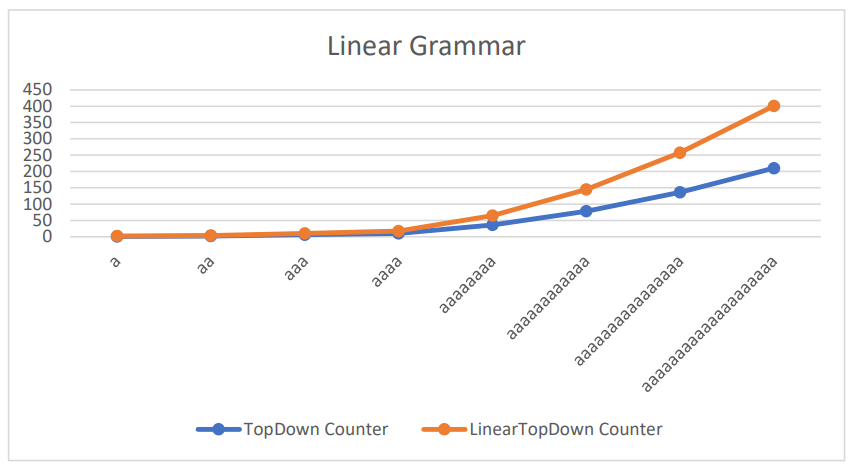
\includegraphics[scale=0.4]{diagrams/LGBTQ.png}
\end{center}
\caption{Linear grammar example (aaa-grammar) on TopDown and linear TopDown parser}
\end{figure}






%---------------------------------------------------------------------%



\subsection{$O$-notation and runtime comparison}
\label{runtime}

% TODO plot graph of runtimes

The runtimes of the methods are calculated in section \ref{systemdesign}. The results are the following:
\ \\ \\
\begin{tabular}{|l|c|}
\hline
Method & Runtime \\
\hline
\texttt{parseNaive} & $O(n!)$\\
\texttt{ParseTD} & $O(n!)$ \\
\texttt{ParseBU} & $O(n^3)$\\
\texttt{ParseLinearTD} & $O(n^2)$\\
\hline
\end{tabular}

\ \\
Seeing those runtimes one could think that the naive and the topdown approach are equally efficient. Considering the differences in the algorithms and the results of the experiments it gets shown that this is not the case. The O-notation runtimes are the upper bounds for the runtime. 

Regarding the experiments that were run on the code, the topdown method seems to be the most efficient, followed by the bottomup method. The least efficient method is in these cases the naive approach.

The linear version of the topdown is more efficient than the original paring method, because it is restricted to linear grammars and with this restriction the recursive calls can be reduced from two to one in each call.

It is to consider that the $O$-notation represents the upper bound of the runtime. Algorithms can run faster than the runtime in $O$-notation predicts.

To confirm the calculated runtimes from Section \ref{systemdesign}, the results of the experiments are calculated, considering the $O$-notation runtime. For the input length ($n$) the actual results and $O$-notation results as upper bound are compared.

\newpage
\textbf{Naive approach ($O(n!)$):} \\
Well-Balanced-Parantheses: 

\begin{tabular}{|c|c|c|}
\hline
$n$ & $n!$ & counter \\
\hline
2& 2 & 6\\
4& 24 & 33\\
6& 720 & 212\\
8& 40.320 & 1295\\
10& 3.628.800 &7666 \\
20& 2.432.902.008.176.640.000 & 51.863.993\\
30& 265.252.859.812.191.058.636.308.480.000.000 & 348.838.486.712\\
\hline
\end{tabular}

Abc-grammar: 

\begin{tabular}{|c|c|c|}
\hline
$n$ & $n!$ & counter \\
\hline
3& 6 & 6\\
4& 24 & 51\\
12& 479.001.600 & 1.457\\
24& 620.448.401.733.239.439.360.000 & 481.557\\
\hline
\end{tabular}

The results of the experiments confirm the runtime calculation of $O(n!)$ in Section \ref{naiveruntime}. Small deviations for smaller input numbers can happen, because the constants are not considered.



\textbf{Topdown approach ($O(n!)$):} \\
Well-Balanced-Parantheses: 

\begin{tabular}{|c|c|c|}
\hline
$n$ & $n!$ & counter \\
\hline
2& 2 & 6\\
4& 24 & 28\\
6& 720 & 84\\
8& 40.320 & 190\\
10& 3.628.800 & 362 \\
20& 2.432.902.008.176.640.000 & 2.772\\
30& 265.252.859.812.191.058.636.308.480.000.000 & 9.232\\
\hline
\end{tabular}

Abc-grammar: 

\begin{tabular}{|c|c|c|}
\hline
$n$ & $n!$ & counter \\
\hline
3& 6 & 6\\
4& 24 & 49\\
12& 479.001.600 & 518\\
24& 620.448.401.733.239.439.360.000 & 6.732\\
\hline
\end{tabular}

The results of the experiments confirm the runtime calculation of $O(n!)$ in Section \ref{topdownruntime}.



\newpage
\textbf{Bottomup approach ($O(n^3)$):} \\

\begin{minipage}{0.5\textwidth}

Well-Balanced-Parantheses: \\

\begin{tabular}{|c|c|c|}
\hline
$n$ & $n^3$ & counter \\
\hline
2& 8 & 6\\
4& 64 & 28\\
6& 216 & 84\\
8& 512 & 190 \\
10& 1.000 & 362 \\
20& 8.000 & 2.772 \\
30& 27.000 & 21.743\\
\hline
\end{tabular}

\end{minipage}\begin{minipage}{0.5\textwidth}
    
Abc-grammar: \\

\begin{tabular}{|c|c|c|}
\hline
$n$ & $n^3$ & counter \\
\hline
3& 27 & 6\\
4& 64 & 49 \\
12& 1.728 & 518\\
24& 13.824 & 4.312\\
\hline
\end{tabular}   
\ \\ \ \\ \ \\  
\end{minipage}


The results of the experiments confirm the runtime calculation of $O(n^3)$ in Section \ref{bottomupruntime}.



\textbf{Linear topdown approach ($O(n^2)$):} 
    
Abc-grammar: 

\begin{tabular}{|c|c|c|}
\hline
$n$ & $n^2$ & counter \\
\hline
3& 9 & 5\\
4& 16 & 51 \\
12& 144 & 650\\
24& 576 & 6.732\\
\hline
\end{tabular}   

The results of the experiments do not confirm the runtime calculation of $O(n^2)$ in Section \ref{lineartopdown}. This is further discussed in Section \ref{results_linear}.



%---------------------------------------------------------------------%
\subsection{Results}
\label{results}

\begin{minipage}{0.5\textwidth}
The $O$-notation results from Section \ref{systemdesign} show, that the naive and the topdown approach have the same upper bound runtime of $O(n!)$ and the bottomup parser has an upper bound runtime in $O(n^3)$.
The experiments on the other hand show, that the topdown approach is a lot 
\end{minipage}
\begin{minipage}{0.1\textwidth} \ \end{minipage}
\begin{minipage}{0.3\textwidth}
\begin{tabular}{|l|c|}
\hline
Method & Runtime \\
\hline
\texttt{parseNaive} & $O(n!)$\\
\texttt{ParseTD} & $O(n!)$ \\
\texttt{ParseBU} & $O(n^3)$\\
\texttt{ParseLinearTD} & $O(n^3)$\\
\hline
\end{tabular}
\end{minipage}


faster than the naive parser. Considering the experiments, the topdown parser seems to be the fastest, followed by the bottomup approach and the naive is by far the slowest.
The parser for linear grammars has different restrictions for the input and its results are discussed in Section \ref{results_linear}.

The reason for the faster results of the topdown parser is the global boolean table, which saves results from previous function calls and can cause less recursive calls of the function to compare the values while the naive approach calls the recursion for every single possibility. The actual runtime of the naive approach is often a lot closer to the upper bound than the actual runtime of the topdown approach, which seems to perform more efficient in the experiments.

In the experiments, the topdown performed even better than the bottomup approach, even though the bottomup parser is in $O(n^3)$. Because the bottomup fills in the CYK-table iteratively, the upper bound runtime is similar to the actual runtime.

For these results it needs to be considered, that the $O$-notation stes the bound from above. An algorithm does not run worse than the depending $O$-notation runtime, but it can be better. It grows at most as much as the $O$-notation function. \cite{bigO}

%---------------------------------------------------------------------%
\subsection{Results for linear grammars}
\label{results_linear}

The upper bound runtime of the modified topdown parser for linear grammars is faster than the runtimes of the parser for grammars in CNF. The topdown runtime is in $O(n!)$ and the modified topdown approach should be in $O(n^2)$. In the linear approach are one instead of two recursive call per execution made, because the linear grammars have at most one nonterminal symbol in the body of each rule. The recursive call needs only to be made for the nonterminal symbols. 
This is why the upper bound runtime if the topdown approach for linear grammars is in $O(n^2)$, while the topdown approach for grammars in CNF is in $O(n!)$.


Surprisingly, the experiments with the modified parsing method do not show the expected results. The linear topdown approach seems to perform faster than the not modified approach, but with more function calls. This seems unlikely, because the recursive calls of the function are reduced from two to one in the modified approach. The faster performance can be due to hidden background processes on the computer. The amount of calls on the other hand should be lower than the amount of calls in the not modified topdown parser. This leads to the assumption, that the modified topdown parser is not working correctly.

The parsing from a linear grammar into CNF works correctly. As seen in the experiments, the input of linear grammars or grammars in CNF have no significantly influence on the runtime of the parsing methods. The naive parser is in both cases called for every option recursively. The bottomup parser iterates in both cases over the whole CYK-table and the topdown parser makes two recursive calls per call.  

%---------------------------------------------------------------------%



%\subsection{Linear grammars}
%\label{_lineargrammars}





\pagebreak


%---------------------------------------------------------------------%








\section{Error correction}
\label{errorcorrection}

Apart from checking if an input word is part of a language, the amount of errors and the correction of those can be interesting.
Two options for the error correction are considered in this section: A symbol can be exchanged or symbols can be deleted. The output for some examples of the error correction can be seen in Appendix \ref{howtousethecode}.

For the error correction the bottomup parser modified, because the CYK-table shows, which substrings lead to which nonterminal symbols, for example the start symbol.





%---------------------------------------------------------------------%
\subsection{Deletion}
\label{deletion}

For the deletion the table of the CYK-algorithm is used. This is described in Section \ref{cyk} and the parsing method for it is explained in Section \ref{bottomupdescription}.
The CYK-table has to contain the start symbol in the entry on the right top corner to conclude that the word is part of the language. To find an accepted word with deletion, the entry with the start symbol which is closest to the right top is searched. 

The concept on how to find the entry in the array that is further on the top right is described here and shown in the pseudo code of the function \texttt{findBestIndeces} in algorithm \ref{alg:fbi}. The function takes two array positions as $(i,j)$ as input and returns the better position in an int array of the length 2.



\begin{center}
\captionof{algorithm}{int[] findBestIndeces(int $i_a$, int $j_a$, int $i_b$, int $j_b$)}\label{alg:fbi}
\begin{algorithmic}[1]
\State $int[] \ betterIndeces \gets new \ int[2]$
\State $int \  indicator_i \gets i_a - i_b$
\State $int \ indicator_j \gets j_b - j_a$
\If{$indicator_i + indicator_j) == 0$}
\State \Comment{both are equal far away}
\State $betterIndeces[0] \gets i_a$
\State $betterIndeces[1] \gets j_a$
\EndIf
\If{$indicator_i + indicator_j) > 0$}
\State \Comment{b is closer}
\State $betterIndeces[0] \gets i_b$
\State $betterIndeces[1] \gets j_b$
\Else
\State \Comment{a is closer}
\State $betterIndeces[0] \gets i_a$
\State $betterIndeces[1] \gets j_a$
\EndIf
\State \Return $betterIndeces$
\end{algorithmic}
\hrulefill
\end{center}


The parameters for the functions are the $i$ and $j$ values for the two positions $A$ and $B$ in the array as $A_i$, $A_j$, $B_i$, $B_j$. The searched position in the array is a small $i$ with a large $j$.

Two values are stored for later comparisons: $x = A_i - B_i$ and $y = B_j-A_j$. If $x$ and $y$ are equal, the positions are equally far away from the top right array entry. If $x+y$ is positive, $B$ is the preferred position, else it is $A$.


With those indices the part of the word that is accepted and the part that needs to be deleted can be calculated. This is done in the method \texttt{solveErrorWithDeletion} which is shown as pseudo code in algorithm \ref{alg:deletion}. This concludes in the longest accepted word with deletion, which is then returned.

It can happen that no accepted word is found with deletion, if no subword concluded into the start symbol in the CYK-table.

The distance of the entry in the CYK-table that contains the start symbol and the top right corner can also be returned as the amount of symbols that need to be deleted to receive an accepted word. This error counter works only for the deletion method.

\begin{center}
\captionof{algorithm}{Integer[] solveErrorWithDeletion(Integer[][][] CYK, int amountOfErrors)}\label{alg:deletion}
\begin{algorithmic}[1]
\State $int \ i \gets -1$
\State $int \ j \gets -1$
\State $int[] \ betterIndeces \gets new \ int[2]$
\For{$index \gets 0$ \textbf{to} $CYK.length$} 
\For{$entries \gets 0$ \textbf{to} $CYK[amountOfErrors][index].length$} 
\If{ $CYK[amountOfErrors][index][entries] == 0$}
\State $betterIndeces \gets findBestIndeces(i, j, amountOfErrors, index)$
\State $i \gets betterIndeces[0]$
\State $j \gets betterIndeces[1]$
\EndIf
\State $temp \gets CYK.length - 1 - amountOfErrors$
\If{$CYK[index][temp][entries] == 0}$
\State $betterIndeces \gets findBestIndeces(i, j, index, temp)$
\State $i \gets betterIndeces[0]$
\State $j \gets betterIndeces[1]$
\EndIf
\EndFor          
\EndFor
\If{$i == -1$}
\State $Integer[] \ noAcceptedWord \gets new \ Integer[1]$
\State $noAcceptedWord[0] \gets -1$
\State \Return $noAcceptedWord$
\EndIf

\State $int \ from \gets Math.min(i, j)$
\State $int \ to \gets Math.max(i, j)$
\State $Integer[] acceptedWord \gets new \ Integer[to - from + 1]$
\If{$from == to$}
\For{$k \gets 1 \textbf{ to } inputAsInt.length$}
\If{$inputAsInt[k] != null \textbf{ and } inputAsInt[k] == 0$}
\State $acceptedWord[k] \gets inputAsInt[k]$
\State $break$
\EndIf
\EndFor
\State \Return $acceptedWord$
\EndIf

\For{$k \gets 1 \textbf{ to } to - from$}
\If{$inputAsInt[k + from] != null$}
\State $acceptedWord[k] \gets inputAsInt[k + from]$
\EndIf
\EndFor
\State \Return $acceptedWord$
\end{algorithmic}
\hrulefill
\end{center}












%---------------------------------------------------------------------%
\subsection{Exchange}
\label{exchange}

The exchange method works iterative and iterates over every symbol of the input word and tries ever terminal symbol on each index. The method can only exchange one symbol. First, the symbol and each entry in the CYK-table that concluded from this symbol in the input word are deleted. For this, the corresponding entries are replaced with $-1$. Then the fields that are assigned with $-1$ in the CYK-table get calculated with a new input symbol, which replaces the original one. 
If a success is found, the accepted word is returned. 

In algorithm \ref{alg:buns} the adapted version of the bottomUp parser can be seen as pseudo code. In this methos, a symbol from the input word got replaced by a new symbol (which is the parameter \texttt{newSymbol}). All the entries, that relied on this symbol were replaced by $-1$ before and this version of the bottomUp parser examines the new entries of these field to produce a full CYK-table for the new input word without calculating the already known parts again.


\begin{center}
\captionof{algorithm}{parseBUnewSymbol(Integer[][][] DP, int newSymbol)}\label{alg:buns}
\begin{algorithmic}[1]
\State $wordlength \gets word.length$ 
\For{$i \gets 0$ \textbf{to} $wordlength$}
\If{$DP[i][i][0] != null \textbf{ and } DP[i][i][0] == -1$}
\State $DP[i][i][0] \gets newSymbol$
\EndIf
\EndFor

\For{$l \gets 0$ \textbf{to} $wordlength$}
\For{$i \gets 0$ \textbf{to} $wordlength - l$}
\State $j \gets i + l$
\If{$DP[i][j][0] != null \textbf{ and } DP[i][j][0] == -1$}
\For{$k \gets 0$ \textbf{to} $j$}

\For{$head \gets 0$ \textbf{to} $ruleset.length$}
\For{$body \gets 0$ \textbf{to} $ruleset[head].length$}
\State $conter \gets counter + 1$
\If{$ruleset[indexNT][bodyIndex][0] \  != null$ \newline \hspace*{5em} \textbf{and} $ruleset[indexNT][bodyIndex][1] \  != null$}
\State $first \gets ruleset[head][body].charAt[0]$
\State $second \gets ruleset[head][body][1]$
\If{$DP[i][k] \ contains \ first$ \textbf{and} $DP[k+1][j] \ contains \ second$}
\State assign head to $DP[i][j][c]$
\EndIf
\EndIf
\EndFor
\EndFor
\EndFor
\EndIf
\EndFor
\EndFor
\If{$DP[0][wordlength-1] \  contains \ 0$}
\State \Return true
\EndIf
\State \Return false
\end{algorithmic}
\hrulefill
\end{center}








%---------------------------------------------------------------------%






\newpage

\section{Conclusion and Future Work}
\label{conclusion}


\subsection{Conclusion}


Regarding the experiments from section \ref{evaluation}, the topdown method seems to be the most efficient, followed by the bottomup method. The least efficient method is in these cases the naive approach. The $O$-notation showed different results considering the upper bounds of the methods. This shows, that the $O$-notation bound is an upper bound and an algorithm can perform faster in experiments, depending on the input stream.


These algorithms show differences in efficiency but also limits for the examination of words with the \textit{CYK}-algorithm. The amount of calls raised especially with the Well-Balanced-Parantheses language exponentially. This can also be seen in the graphs in Appendix \ref{graph}.

The linear parsing method on the other hand worked with a different restriction on the input stream, which can lead into even higher performances.


\subsection{Future work}

Formal languages and grammars can be used in different use cases. For exampel for AI learning methods. Real languages like English can be defined as a formal language, too. But it is important to consider that formal languages only define the syntax and not the semantics. In addition to this has english a lot of rules and many exceptions. \cite{FG}

The future work for this code is to optimize the error correction. The combination of deletion and exchange is not implemented yet. It would be interesting to find a more efficient way to calculate the exchange of symbols, which would enable the exchange of more than one symbol.
In addition to this an accurate error counter for the symbols that need to be exchanged could be implemented.

Another extension to the code would be a method, that translated every kind of grammar into \textit{CNF}, if possible. Then input words for every grammar could be parsed with the different parsing approaches and possibilities to modify the parsing methods for different input grammars appear, similar to the modifications that were done for the parsing of linear grammars.


% The future work for this assignment is to change the types of the arrays from \texttt{String[][]} to \texttt{int[][][]}. In addition to this there still exists a problem in the bottomup method, which needs to be fixed. Some specific grammars and words do not return the right value. After these things work correctly, more experiments can be run and the pseudo code will be edited. Then the upper bound runtime can be calculated again and the plotted graphs can be compared to the according $O$-notation runtime.


\newpage





%---------------------------------------------------------------------%






%---------------------------------------------------------------------%
\newpage

\fancyhead[LO]{\empty}





\phantomsection
\addcontentsline{toc}{section}{\bibname}
%\begin{spacing}{1.3}
\printbibliography
%\end{spacing}



%---------------------------------------------------------------------%

\newpage

\appendix

\section{How to use the code?}
\label{howtousethecode}

The code can be run in the terminal and input is expected as Strings in quotation marks. The first rule begins with the startsymbol of the grammar. \\ \\
First: Rules without arrows (one rule as one String) \\
Last: The last argument is the input word
\\ 
Input example (\textit{Well-Balanced-Parantheses}):\\
  \texttt{java Main \dq SSS\dq \ \dq SLA\dq \ \dq SLR\dq \ \dq ASR\dq \ \dq L(\dq \ \dq R)\dq\  \dq (())\dq} \\
  for the grammar \texttt{S $\rightarrow$ SS | LA | LR, A $\rightarrow$ SR, L $\rightarrow$ (, R $\rightarrow$ )} and the input word \texttt{(())}. \\
Other example: \\
 \texttt{java Main \dq SAc\dq \ \dq Sb\dq \ \dq AaS\dq \ \dq AaB\dq \ \dq BbS\dq \ \dq abc\dq } 
\\ 
\\
Output example: \\
The first part of the output shows the arrays, which get generated in the \texttt{Grammar.java} class.  \\ \\
\begin{minipage}{0.6\textwidth}
\vspace*{-2em}
\ \\
The first array contains all rules. \\ \\

The second array contains only the terminal rules. \\ \\

The third array contains only the nonterminal rules. \\

Then it is shown which symbols are represented by which integers. Later the symbols can be referred to with those integers. \\ 

After this the mentioned arrays are shown again but the nonterminal symbols got replaced with the according integers. \\ \\

Then the input word is shown with the symbols replaced by their integers.

\end{minipage}\begin{minipage}{0.1\textwidth}
\ 
\end{minipage}\begin{minipage}{0.3\textwidth}
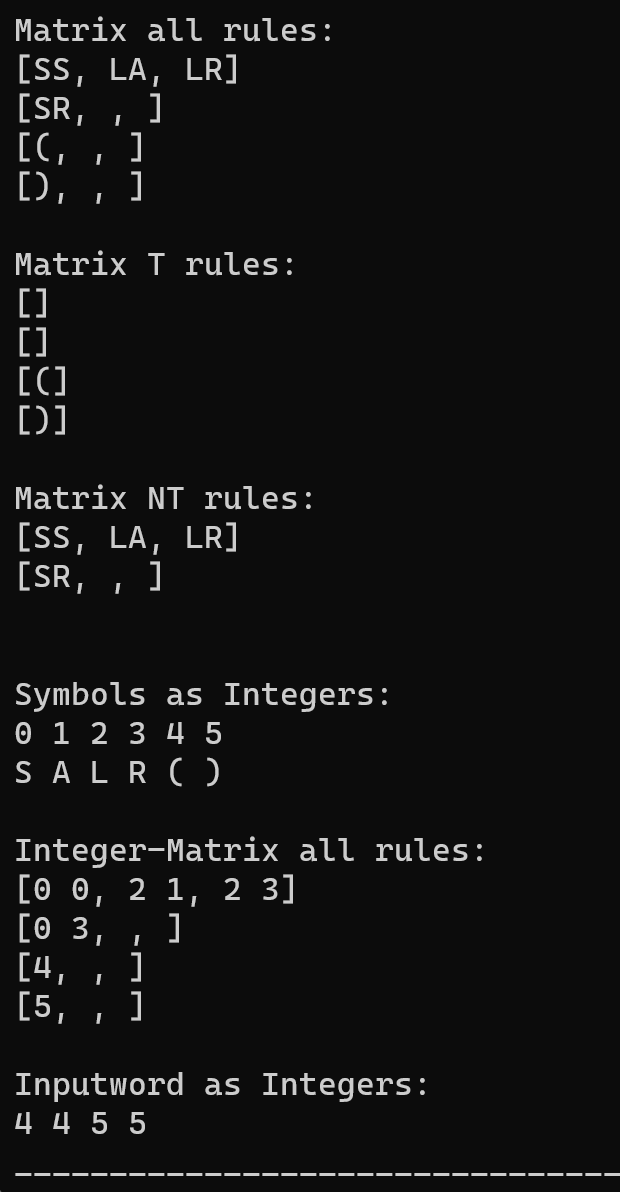
\includegraphics[scale=0.7]{images/terminal_1.png}
\end{minipage}

\begin{minipage}{0.6\textwidth}
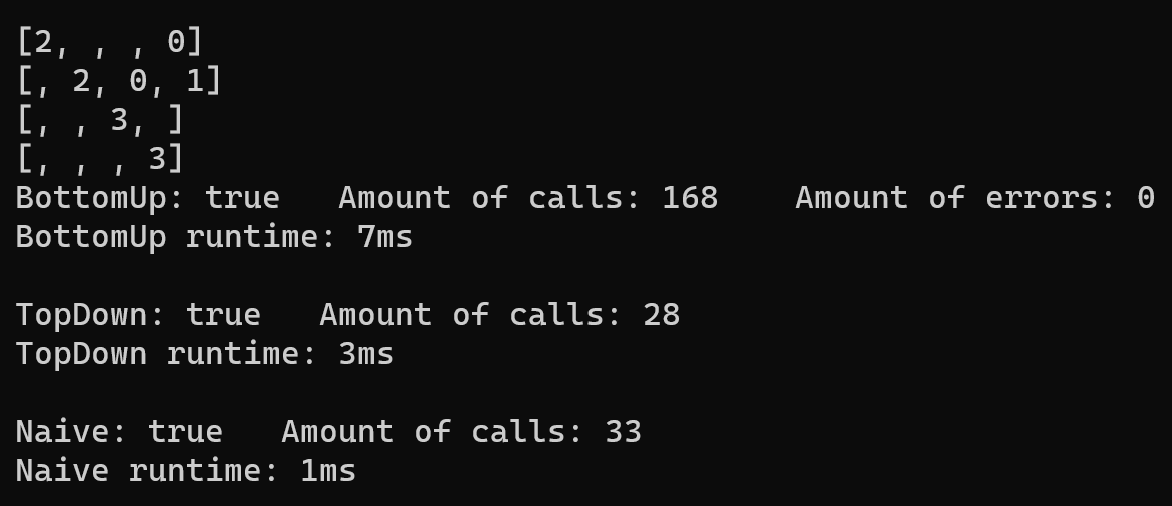
\includegraphics[scale=0.6]{images/terminal_2.png}
\end{minipage}\begin{minipage}{0.1\textwidth}
\ 
\end{minipage}\begin{minipage}{0.3\textwidth}
Then the results, counter and runtime in $ms$ is shown for each parsing method. \\
For the \texttt{BottomUp} method is the CYK algorithm table printed.
The error counter is printed, too.
\end{minipage}

\begin{minipage}{0.35\textwidth}
In this case the error correction shows that no errors where found and this leads to no symbols being exchanged or deleted.

\end{minipage}\begin{minipage}{0.1\textwidth}
\ 
\end{minipage}\begin{minipage}{0.55\textwidth}
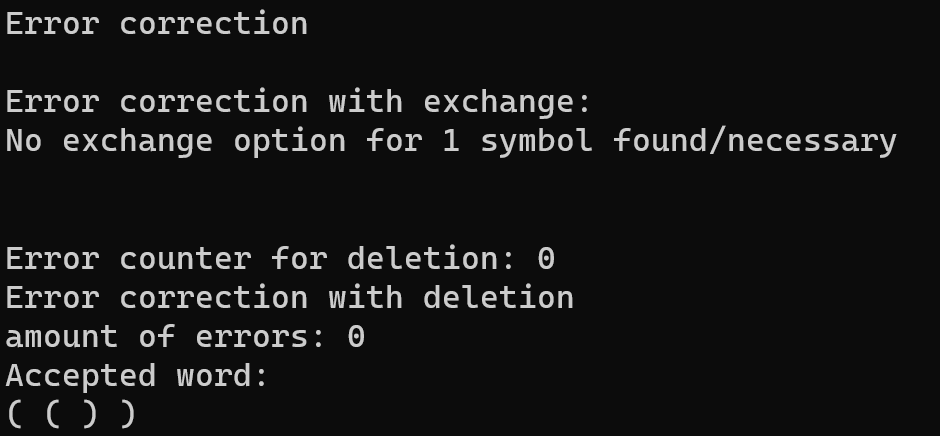
\includegraphics[scale=0.7]{images/terminal_3.png}
\end{minipage}

\ \\
The following example shows the error correction output for the input \texttt{java Main \dq SSS\dq \ \dq SLA\dq \ \dq SLR\dq \ \dq ASR\dq \ \dq L(\dq \ \dq R)\dq\  \dq ((()\dq}. \\

\begin{minipage}{0.35\textwidth}
In this case the error correction shows the solution with exchange (one symbol is exchanged) and for deletion (two symbols are deleted).

\end{minipage}\begin{minipage}{0.1\textwidth}
\ 
\end{minipage}\begin{minipage}{0.55\textwidth}
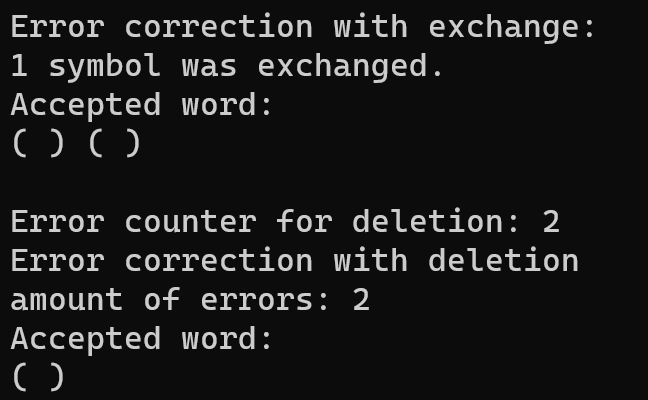
\includegraphics[scale=0.7]{images/terminal_4.png}
\end{minipage}

\begin{minipage}{0.5\textwidth}
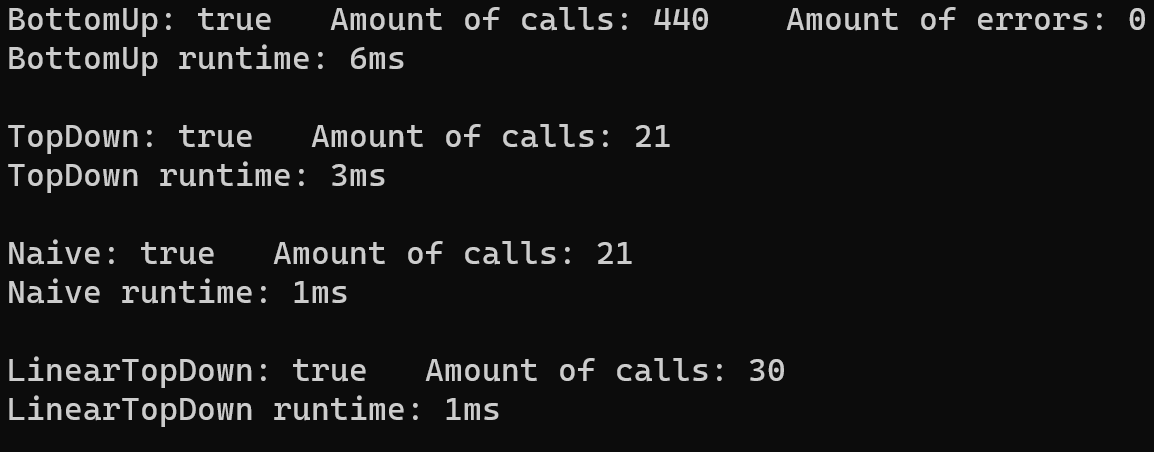
\includegraphics[scale=0.55]{images/terminal_5.png}
\end{minipage}\begin{minipage}{0.1\textwidth}
\ 
\end{minipage}\begin{minipage}{0.4\textwidth}
If the input grammar is a linear grammar, the program checks if it is in \textit{CNF}, build \textit{CNF} out of the linear grammar and runs the optimized version of the TopDown parser for linear grammars.
\end{minipage}





%---------------------------------------------------------------------%







% \newpage
% \section{Graphs and additional results}
% \label{previousresults}










%---------------------------------------------------------------------%







\newpage
\section{CNF Algorithm on an example}

% \subsection{CNF Algorithm on an example}
\label{createcnf}

In this part, the following ruleset of a grammar is translated into \textit{CNF}.

\begin{align*}
\texttt{S} & \rightarrow \texttt{SS} \mid  \texttt{aSb} \mid \texttt{ab} 
\end{align*}

\begin{enumerate}

\item Remove every nonterminal symbol that cannot be reached or is not generating another symbol: \\
\texttt{S} is the only nonterminal symbol and does not need to be removed.

\item Remove all symbols that cannot be reached. (All symbols can be reached.)

\item Replace the terminal symbols in the body of other rules with new nonterminal symbols to not have bodies which contain terminal and nonterminal symbols:
\begin{align*}
\texttt{S} & \rightarrow \texttt{SS} \mid  \texttt{LSR} \mid \texttt{LR}  \\
\texttt{L} & \rightarrow \texttt{a} \\
\texttt{R} & \rightarrow \texttt{b} 
\end{align*}


\item On the right side of the rules are only two nonterminal symbols allowed:
\begin{align*}
\texttt{S} & \rightarrow \texttt{SS} \mid  \texttt{LA} \mid \texttt{LR}  \\
\texttt{A} & \rightarrow \texttt{SR} \\
\texttt{L} & \rightarrow \texttt{a} \\
\texttt{R} & \rightarrow \texttt{b} 
\end{align*}

\item Remove all $\epsilon$-rules and paste in the start symbol what can be generated by them. (This grammar does not have $\epsilon$-rules.)

\item Check on transitivity and remove those dependencies. (There are no transitive rules here.)

\end{enumerate}

This is the grammar in CNF:
\begin{align*}
\texttt{S} & \rightarrow \texttt{SS} \mid  \texttt{LA} \mid \texttt{LR}  \\
\texttt{A} & \rightarrow \texttt{SR} \\
\texttt{L} & \rightarrow \texttt{a} \\
\texttt{R} & \rightarrow \texttt{b} 
\end{align*}









\end{document}